
\documentclass[titlepage]{article}

\usepackage{graphicx}
\usepackage{longtable}
\usepackage{float}
\usepackage{subfig}
\graphicspath{ {./images/} }
			

\title{{\Huge {\it Data4Help}}}
\author{Lorenzo, Molteni, Negri}
\date{November 11, 2018}

\begin{document}

\makeatletter
    \begin{titlepage}
        \begin{center}
            
\includegraphics[width=\linewidth]{logo.png}\\[20ex]
            {\huge  \@title }\\[2ex] 
            {\LARGE  \@author}\\[3ex] 
            {\LARGE {\it RASD} Document}\\[3ex]
            {\large \@date}\\[5ex]
        \end{center}
    \end{titlepage}
\makeatother
\thispagestyle{empty}
\newpage

%Add content for page two here (useful for two-sided printing)
\thispagestyle{empty}
\newpage


	
%Index	
\pagebreak
\tableofcontents{}
\pagebreak


%Introduction
\section{Introduction}
The following RASD aims at providing an overview of the project {\it Data4Help}. This document will guide the reader in understanding the purpose of the project, on which grounds it is set and in which environment it will live. Precisely, it will illustrate both informally and formally which are the goals and how these may be reached by guaranteeing certain functional and nonfunctional requirements, while certain phenomena hold in the world.
The document will provide a baseline for the project’s planning and estimation and will support the software’s evaluation. 
Finally, it will be the starting point for the software’s review and update.
The document is addressed to all those who intend to benefit from the service and who may be involved in its development. 

	
	\subsection{Purpose}
{\it Data4Help} is a service that aims at keeping track of individuals’ health conditions. The application’s goal is achieved by allowing individuals to share their position and health data and by enabling {\it Third Parties} to request and monitor them. 
{\it Single User}s will enjoy a clear summary of their health status and will feel safe by being continuously monitored by {\it Third Parties}. {\it Third Parties}, on the other hand, will have direct access to users’ data and will be able to use them to perform analysis for medical purposes. \\
\\
{\it Data4Help} requires the user to create an account to access its services, the functionalities unlocked after registration depend on the type of account created.\\
If a user creates an account as a “{\it Single User}”, he/she will be asked to provide some basic information, precisely name, last name and date of birth. Furthermore, he must provide an email with which he will be uniquely identified, a password and a fiscal code. When all the registration requirements are fulfilled, a user will have activated his personal account. However, he will only enjoy of the application’s service once he allows access to his health data and location, imported from his devices.
The user can finally visualize a summary of his health conditions and reject or accept {\it Third Party} requests asking for his data. The application also allows users to keep track of how many and which {\it Third Parties} are monitoring him.\\
\\
On the other hand, a company will create a “{\it Third Party}” account and will need to provide its name, its P.IVA, a password and, as for private users, will be uniquely identified by an email.  \\
{\it Third Parties} can use the application to collect data in two ways. Firstly, they can retrieve data of a specific individual, identified by a fiscal code or an email, provided that the user responds positively to the request. The {\it System} also allows {\it Third Parties} to subscribe to new data and receive it as soon as it is produced. \\
Secondarily, {\it Third Parties} may also retrieve data concerning groups of users by performing group requests, provided that the filtered result satisfies certain constraints. These requests won’t require the involved users’ approval and will provide anonymous results.\\
\\
In addition to these functionalities, {\it Data4Help} allows {\it Single User}s to activate {\it AutomatedSOS}. This integrated service adds up as another feature preserving the users’ safety. Whenever a user’s health status results critical according to certain thresholds, if {\it AutomatedSOS} is enabled an ambulance is immediately called and sent to his location.\\
\\
{\it Data4Help} offers to its customers also an additional service: {\it Track4Run}. While relying on the solid architecture of {\it Data4Help}, this feature can be accessed by downloading its exclusive application. When a user downloads {\it Track4Run} he will login with his {\it Data4Help} account or will easily register to it at the moment. Those who will access {\it Track4Run} are runners, run organizers and {\it Spectator}s. This application is intended to enable {\it Third Parties} to organize runs, {\it Single User}s to join them and {\it Spectator}s to keep track of runners live during an active path. While runners will enjoy visualizing their position live in the path, organizers will be able to track all participants and, thanks to {\it Data4Help}’s underlying services, will access the runners’ health data. {\it Spectator}s won’t need to create any account as they will simply scroll through the list of active runs and track the runners’ positions in the selected path.\\
\\
From this brief description of the functionalities we may extract the following goals for {\it Data4Help}: \\
		
		\begin{itemize} %GOALS

   			 \item {\bf [G1]} Users can be identified either as {\it {\it Single User}s} or as {\it Third Parties}.				
			 \item {\bf [G2]} {\it {\it Single User}s} can have their data monitored by {\it Third Parties} for medical purposes.
   			 \item {\bf [G3]} {\it {\it Single User}s} can visualize a summary of their health status.
   			 \item {\bf [G4]} {\it Third Parties} can access data of those {\it Single User}s who granted their permission.
   			 \item {\bf [G5]} {\it Third Parties} can access data of anonymous groups of users. \\
			 \\
With regards to {\it {\it AutomatedSOS}}, we may identify one goal: 
   			 \item {\bf [G6]} Whenever a user’s health status becomes critical, an ambulance is sent to his location. \\	
			 \\
 Finally, for {\it Track4Run}, we extract the following goals:
			  \item {\bf [G7]} Organizers can create and manage runs.
			  \item {\bf [G8]} Runners can enroll in an existing run.
			  \item {\bf [G9]} {\it Spectator}s can track the position of runners during a run.
			\end{itemize}
			
	\subsection{Scope}
Following the definition originally proposed by M. Jackson and P. Zave in 1995, we will try to clarify the scope and the application range of the {\it System} by identifying the so called World and Machine phenomena.\\
The Machine is the {\it System} to be developed, in this case a software, while the World, also known as environment, corresponds to the part of the real world that is affected by the {\it System}. \\
The World and the Machine are associated with different types of events which we are going to describe and detail.
World and the Machine are associated with different types of events which we are going to describe and detail.\\		
		\subsubsection{World Phenomena}
		World phenomena are events that take place in the real world and taken by themselves do not have a direct impact on the {\it System}.\\
We identify the following world phenomena:
		\begin{itemize}
			\item Heart rate of a {\it Single User} drops due to a stroke.
			\item A user has an accident.
			\item A user is in an extreme physical condition.
			\item A user changes his location.
			\item A user has a regular heart rate.
			\item A user performs some kind of physical activity.
			\item A user takes part in a run.
		\end{itemize}

		\subsubsection{Shared Phenomena}
		Shared phenomena are world phenomena that are shared with the Machine.\\
These are further divided in two categories: phenomena controlled by the World and observed by the Machine and phenomena controlled by the Machine and observed by the World.\\
With regard to the first kind we identify the followings:
		\begin{itemize}
			\item A user inputs to the {\it System} all data needed for registration.
			\item A user’s health data is collected into the {\it System}.
			\item A user sends a data request to the {\it System}.
			\item A user enables {\it AutomatedSOS}.
			\item A user joins an active run.
			\item A user checks-in a run he previously joined.
			\item A user organizes a run.\\
		\end{itemize}
Concerning the second type:	
		\begin{itemize}
			\item A user visualizes his health status.
			\item The {\it System} shows the result of a request.
			\item The {\it System} forwards a request notification to a user.
			\item The {\it System} asks a runner to share his data.
			\item The {\it System} shows to all {\it Spectator}s a user’s position during a run.
			\item The {\it System} shows data of participants of a run to its organizer.
		\end{itemize}	
		
		\subsubsection{Machine Phenomena}
		Machine phenomena are events that entirely take place inside the {\it System} and cannot be observed in the real world.\\
We identified:
		\begin{itemize}
			\item Retrieving result data for a request.
			\item Storing permanently collected data.
			\item Encryption of sensitive data.
		\end{itemize}

	\subsection{Definitions, Acronyms, Abbreviations}
		
		\subsubsection{Acronyms}
	
		\begin{longtable}{| p{2 cm} | p{7 cm} |} \hline
			{\bf S2B} & {\it System} to be \\\hline
			{\bf GDPR} & General Data Protection Regulation \\ \hline
			{\bf GPS} & Global Positioning {\it System} \\ \hline
			{\bf API} & Application Programming Interface \\ \hline
			{\bf FC} & Fiscal Code \\ \hline
			{\bf P.IVA} & Partita IVA \\ \hline
			{\bf BPM} & Beats Per Minute \\ \hline
			{\bf Kcal} & Kilocalories \\ \hline
			{\bf UI} & User Interface \\ \hline
			{\bf WP} & World Phenomena \\ \hline
			{\bf MP} & Machine Phenomena \\ \hline
			{\bf ID} & Identifier \\ \hline
				
			\caption{Acronyms}	
						
		\end{longtable}
			
		\subsubsection{Definitions}
			
			\begin{itemize}
				\item {\bf S2B: } the {\it System} to be developed. It includes both {\it Data4Help} and {\it Track4Run}.
				 \item {\bf Historical Data:} all data provided to the S2B by the user since his registration.
				\item{\bf Active Energy:} Energy consumed by the user when not standing still, measured in Kcal.
				\item{\bf Resting Energy:} Energy consumed by the user when standing still or resting, measured in Kcal.
				\item{\bf Health parameter: } health feature imported from the user’s device, namely weight, height, heart rate, stand hours, active and resting energy, sleeping hours, walking and running distance.
				\item{\bf Health status: } the set of all health parameters, modelling the health of the user at a given time.
				\item{\bf  Group request:} how a {\it Third Party} interacts with the S2B to obtain anonymized data from a group of users.
				\item{\bf Single request: } how a {\it Third Party} interacts with the S2B to obtain data from a {\it Single User}.
				\item{\bf Search parameters:} parameters used to filter users in a group request, such as age, location (address or selected area), values of users’ health parameters.
				\item{\bf Requested data types: } health parameters that {\it Third Parties} want to obtain from users when submitting a request.
				\item{\bf Sensitive Data:  } information that is not provided to {\it Third Parties} when answering a multiple request to guarantee anonymity. This includes position, FC and email.				
				\item{\bf Time series: } cartesian plot of the evolution of a health parameter in time. X axis is a time scale, Y axis is the value of the parameter.
				\item{\bf Statistical operators:} aggregated statistical operators such as Mean, Median, Percentiles, Variance, Standard Deviation and Error.		
				\item{\bf Fiscal code: } a 16 characters code used in Italy to uniquely identify a citizen.
				\item{\bf Partita IVA: } a 11 characters code used in Italy to uniquely identify a company for value added tax purposes (VATIN in Europe).
				\item{\bf Credentials: } the email and password provided during registration.
				\item{\bf Joining a run: } expressing the non-binding intention to take part in a run.
				\item{\bf Check-in: } binding confirmation that a user will take part in a run, agreeing to share his data			\end{itemize}
				
				
		\subsubsection{Abbreviations}
			
			\begin{itemize}
				\item {\bf (Gn):} n-th Goal
				\item {\bf (Rn):} n-th Requirement
				\item {\bf (Dn):} n-th Domain Assumption
				\item {\bf (Cn):} n-th Constraint
				\item {\bf SP1:} shared phenomena controlled by the World and observed by the Machine
				\item {\bf SP2:} shared phenomena controlled by the Machine and observed by the World
				\item {\bf WP:} World Phenomena 
				\item {\bf MP:} Machine Phenomena
			\end{itemize}
			
	\subsection{Revision History}
	
	\begin{table}[ht]
		\centering
		\begin{tabular}{ccc} 
		Version & Date & Changes  \\ 
		\hline
		1.1 & 24/10/2018 & Initial draft \\
		1.2 & 10/11/2018 & First deadline draft \\
		\end{tabular}
		\caption{Revision History}
		\label{default}
	\end{table}
	
	\subsection{Reference Documents}
		
		\begin{itemize}
   			\item ISO/IEC/IEEE 29148: https://www.iso.org/standard/45171.html

   			 \item Alloy Official Documentation: http://alloy.lcs.mit.edu/alloy/documentation.html
   			 \item Four Dark Corners of Requirements Engineering – Jackson, Zave
			 \item Project Assignment
			\end{itemize}

	\subsection{Document Structure}
			The rest of the document is organized as follows:
				\begin{itemize}
					\item {\bf Overall Description} (Section 2) contains an in-depth description of the domain under analysis, following the Jackson-Zave approach used in the Scope paragraph in Section 1. Class Diagrams will be hereby provided to formalize all the actors involved in the {\it System} and their relations, while their needs and scope as Stakeholders will be analyzed later in the section.\\
Key functional requirements will then be listed, together with all the Domain Assumptions that can be used to entail each Goal.
					\item In the {\bf Specific Requirements} (Section 3) functional requirements are associated to use cases and Sequence Diagrams to clarify processes and interactions between users and the S2B. Nonfunctional requirements are also included here, together with external constraints (mainly regulations) imposed on the {\it System}.\\
Developers can also find requirements regarding External Interfaces, with a focus on Hardware and Software Interfaces. Finally, a brief overview of the properties that the S2B will have to guarantee is provided.
					\item {\bf Formal Analysis} (Section 4) uses Alloy to generate a formal model of two distinct parts of {\it Data4Help}, the identification and requests.
				\end{itemize}

\pagebreak	
	
%Overall Description
\section{Overall Description}
	\subsection{Product perspective}
	In this section we will explain in more detail the various World, Machine and shared phenomena. We will also provide 	some of the descriptions with State and Class Diagrams.\\ \\
	{\bf Heart rate of a Single User drops due to a stroke (WP) }\\ 
	In the unlikely situation in which the user is subject of a severe heart attack, his heart rate will suddenly drop under the 	minimum threshold. The same applies for any other medical condition that can arise such as low heart rate due to low 	blood pressure.\\ \\
	{\bf A user has an accident (WP)}\\
	The user may get involved in some kind of accident, for example getting in a car crash or being wounded as a result of 	a work incident. In such cases the user’s biological parameters may vary indicating a critical health condition.\\ \\
	{\bf A user is in an extreme physical condition (WP)}\\
	If the user is performing extremely demanding physical tasks that are exceeding his body capabilities, such as running 	too fast or for too long, ascending a steep cliff or lifting heavy loads, his heart rate may rise too much and put him in 		danger.\\ \\
	{\bf A user changes his location (WP)} \\
	During the course of his daily routine the user usually moves between different areas and locations modifying his 		current position.\\ \\
	{\bf A user has a regular heart rate (WP)} \\ 
	In conditions of healthiness and well being, while no particular physical tasks are performed, the heart rate of the user 	normally lies in the safe interval indicated for is age range.\\ \\
	{\bf A user takes part in a run (WP)}\\
	A user that enjoys running or jogging may decide to participate to an organized run. An organized run usually takes 		place in a specific location at a given time and could allow the enrollment of both amateurs and professionals. \\ \\
	{\bf A user inputs to the System all data needed for registration (SP1)} \\
	During the registration phase the user must provide some mandatory informations such as email, password, FC and 	birthdate. These infos are sent through the {\it System} which takes care of validating and storing them in a new 		account.\\ \\
	{\bf A user’s health data is collected into the System (SP1)} \\
	Granting access to health parameters and location is an essential step towards the exploitation of the {\it System}’s 		potentials. This data is collected by the machine, associated with the user of origin, and stored into a database.\\ \\
	{\bf A user sends a group request to the System (SP1)} \\
	A {\it Third Party} can send a group request to the {\it System} in order to retrieve anonymized data about a group of 		users, filtered with search parameters. The group request is provided as input through the user interface and processed 	internally.\\ \\
	{\bf A user enables AutomatedSOS (SP1)} \\
	At a certain point in time a {\it Single User} may decide to enable {\it AutomatedSOS}, which is an additional feature 		offered by {\it Data4Help}. In order to do so, he has to press a button on the user interface. The {\it System} registers 	the input and enables {\it AutomatedSOS} functionality.\\ \\
	{\bf A user joins an active run (SP1)} \\
	A user who wishes  to participate to a run organized by {\it Track4Run} can either find it by inputting the run’s ID or by 	looking for it in the list of active runs on the {\it System} UI. He then press a button and sign up for the event. The {\it 	System} is alerted and adds that user to the list of participants. \\ \\
{\bf A user checks-in a run he previously joined (SP1)}
When the time of an organized run comes, all participants confirm their presence by giving permissions to share their health and position data with the {\it System}. After a user grants this access, the machine starts collecting and processing its data.\\ \\
{\bf A user organizes a run (SP1)}\\
The user can organize a run by selecting the relative view on the UI and filling all the required fields. All information is received by the {\it System} who proceeds to create a new active run visible to all other users.\\ \\
{\bf The System shows to the user his health status (SP2)} \\
The {\it System} retrieves both current and historical health data related to the user and proceeds to show them in an organized and aggregated way on the user interface.\\ \\
{\bf The System shows the result of a group request (SP2)} \\
After processing a group request, if some results have been obtained from the DBMS, the {\it System} shows the anonymized data to the requesting party in a neat, organized and aggregated way.\\ \\
{\bf The System forwards a request notification to a user (SP2)} \\
After receiving a request from a {\it Third Party} the {\it System} checks if the user specified in the parameters exists and if so proceeds to forward a notification request to him. The notification includes the generalities of the requesting {\it Third Party}, the type of request (subscription or not) and the kinds of health parameters asked.\\ \\
{\bf The System asks a runner to share his data (SP2)}
When the time of a run comes, the {\it System} sends a notification to all users asking for their permission to share Position and Health data.\\ \\
{\bf The System shows to all {\it Spectator}s a user’s position during a run (SP2)} \\
During a run the {\it System} constantly update its internal state with the position of all participants using the data they share. This information is then used to show to {\it Spectator}s where each runner is located using a map on the UI.\\ \\
{\bf The System shows data of participants of a run to its organizer (SP2)} \\
The {\it System} constantly shows to an organizer data about the participants enrolled in a run he created. Said data includes the number of runners, their generalities and after the run starts their position and health data. \\ \\
{\bf Retrieving result data for a group request (MP)} \\
When a group request is received, the {\it System} extracts the filtering parameters and forwards the query to its database. The DBMS extracts all data that satisfies the query. If the results match less than 1000 accounts they are discarded and a failure notification is generated. Otherwise the result is sent to the requesting {\it Third Party}. Furthermore the data is anonymized, which means that all sensible information related to the respective users is hidden. \\ \\
{\bf Storing permanently collected data (MP)} \\
All data collected from registered users is sent to an internal database. The {\it System} makes sure that all this data is not lost or corrupted in any way by using the functionalities provided by a DBMS.\\ \\
{\bf Encryption of sensitive data (MP)} \\
All sensitive data are encrypted by the {\it System} in order to guarantee the privacy of the users in case of malicious attacks or data leaks. Privacy is a big issue in this project because the Machine deals with personal data.\\

		\subsubsection{Class Diagrams}
		
		\begin{figure}[H]
			\center
  			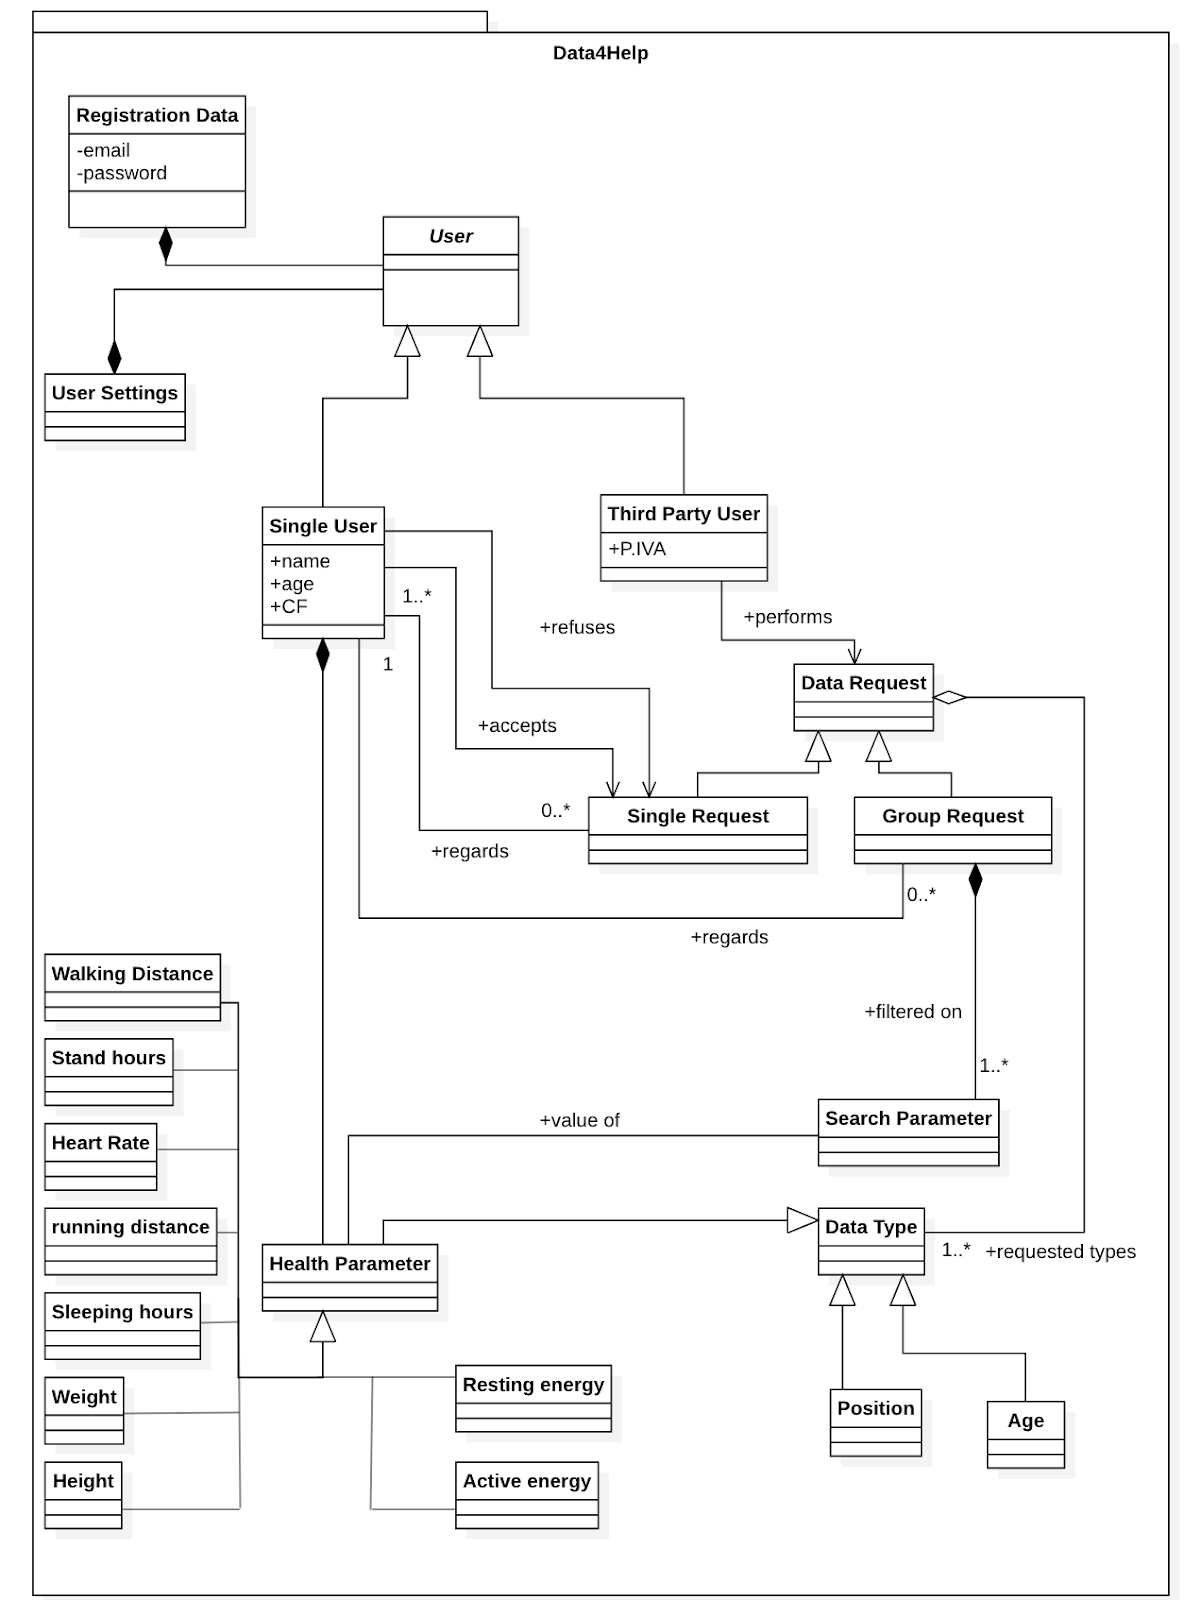
\includegraphics[width=\textwidth]{Diagrammi/D4HClass.png}
  			\caption{{\it Data4Help} Class Diagram}
 			\label{fig:D4HClass}
		\end{figure}
		\begin{figure}[H]
			\center
  			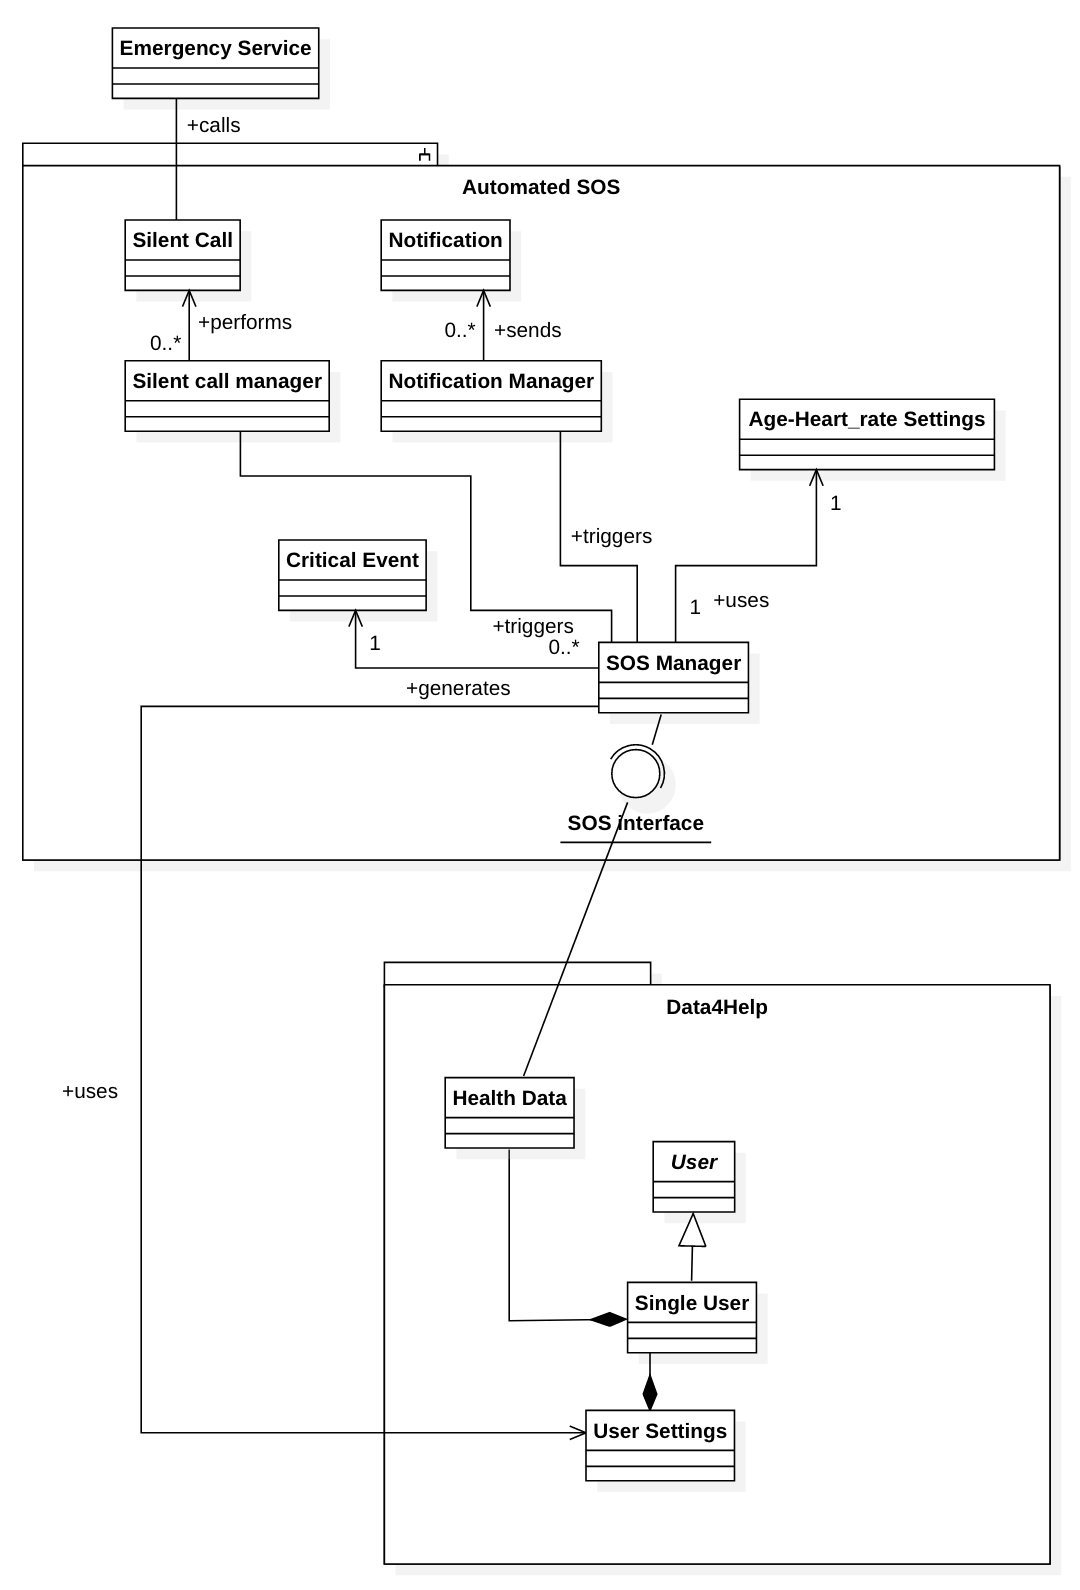
\includegraphics[width=\textwidth]{Diagrammi/SOSClass.png}
  			\caption{{\it AutomatedSOS} Class Diagram}
 			\label{fig:SOSClass}
		\end{figure}
		\begin{figure}[H]
			\center
  			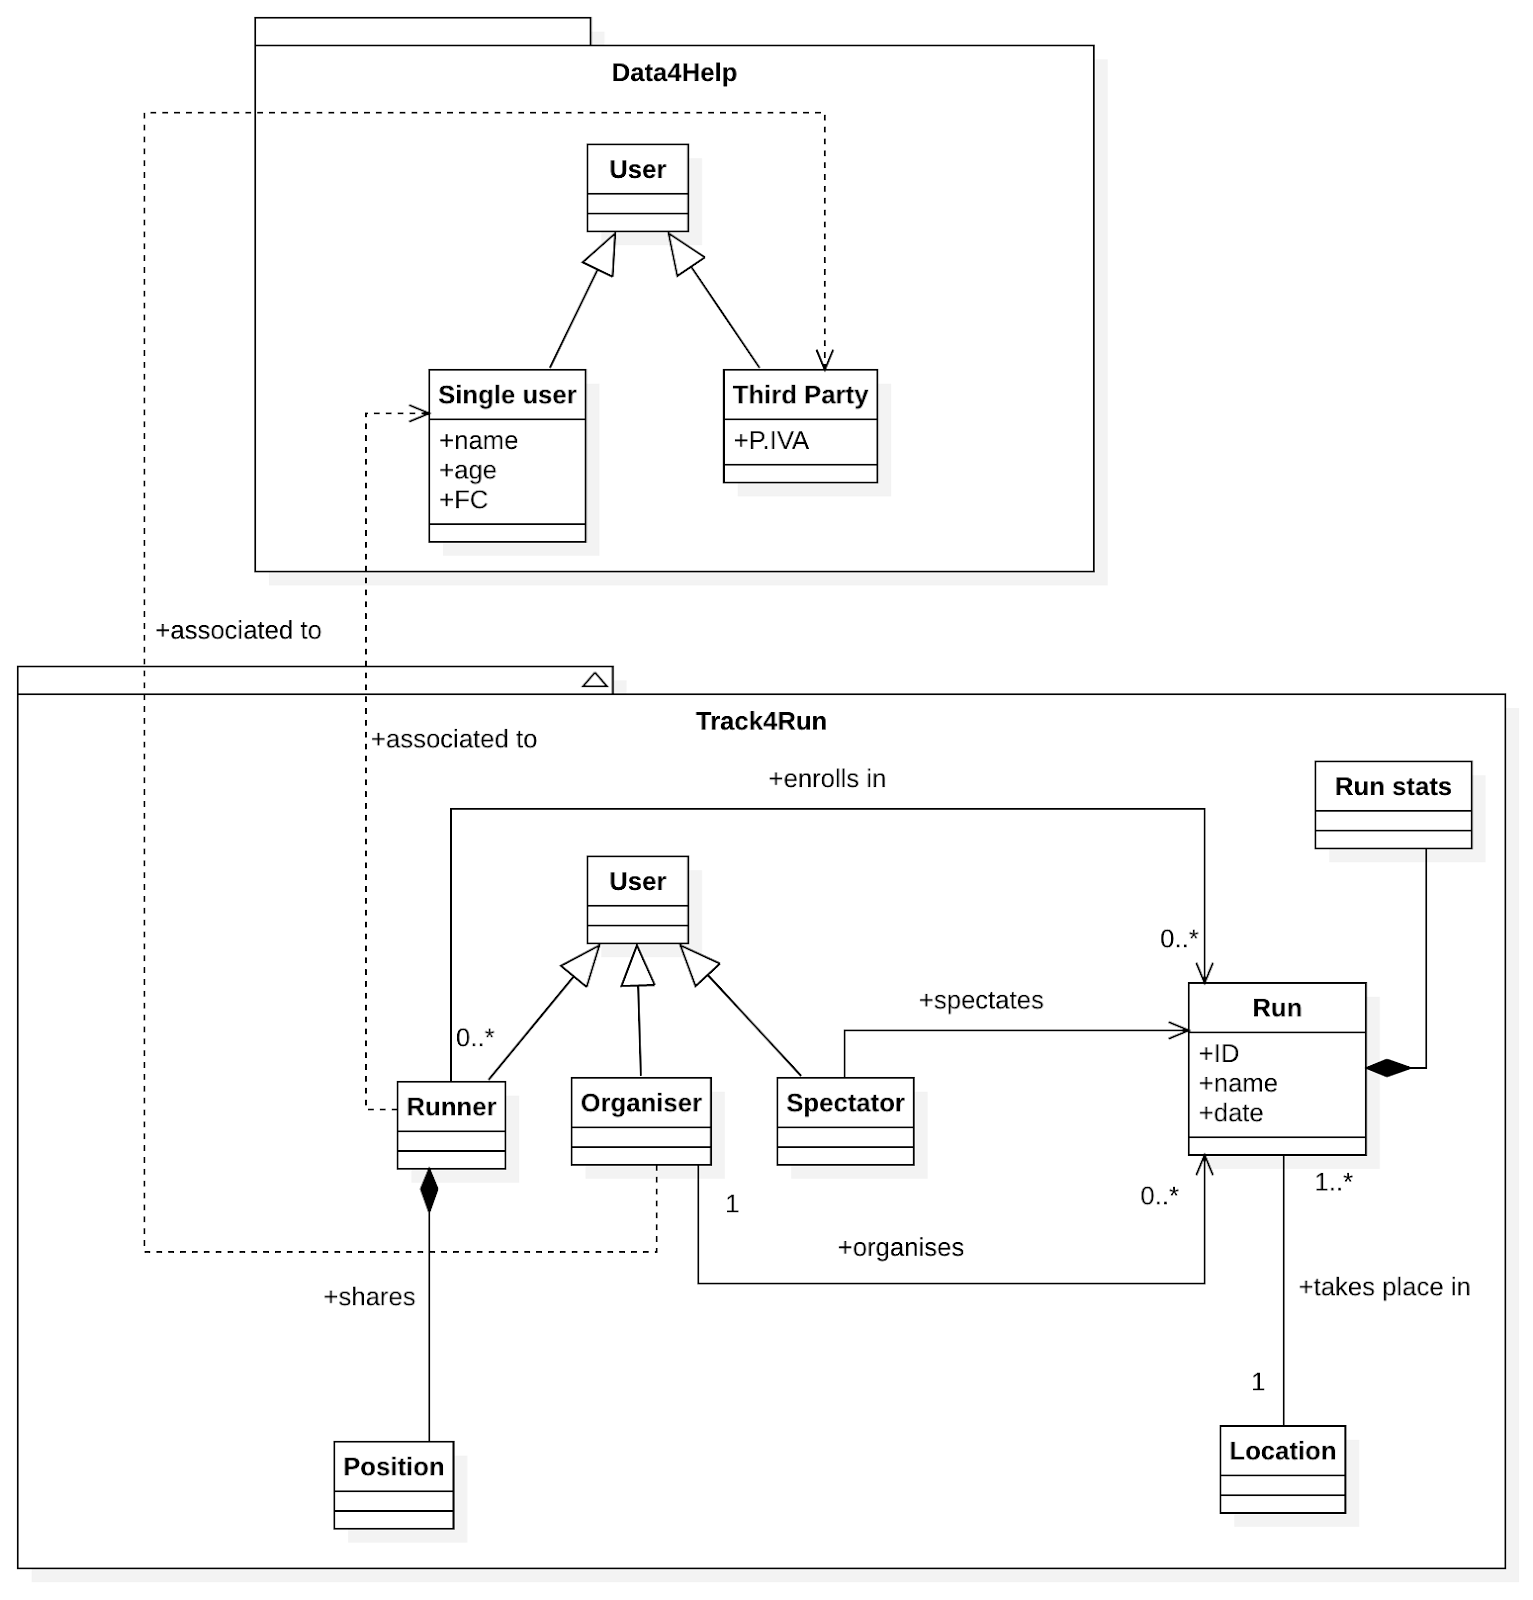
\includegraphics[width=\textwidth]{Diagrammi/T4RClass.png}
  			\caption{{\it Track4Run} Class Diagram}
 			\label{fig:T4RClass}
		\end{figure}
		
		\subsubsection{State Charts}
		\begin{figure}[H]
			\center
  			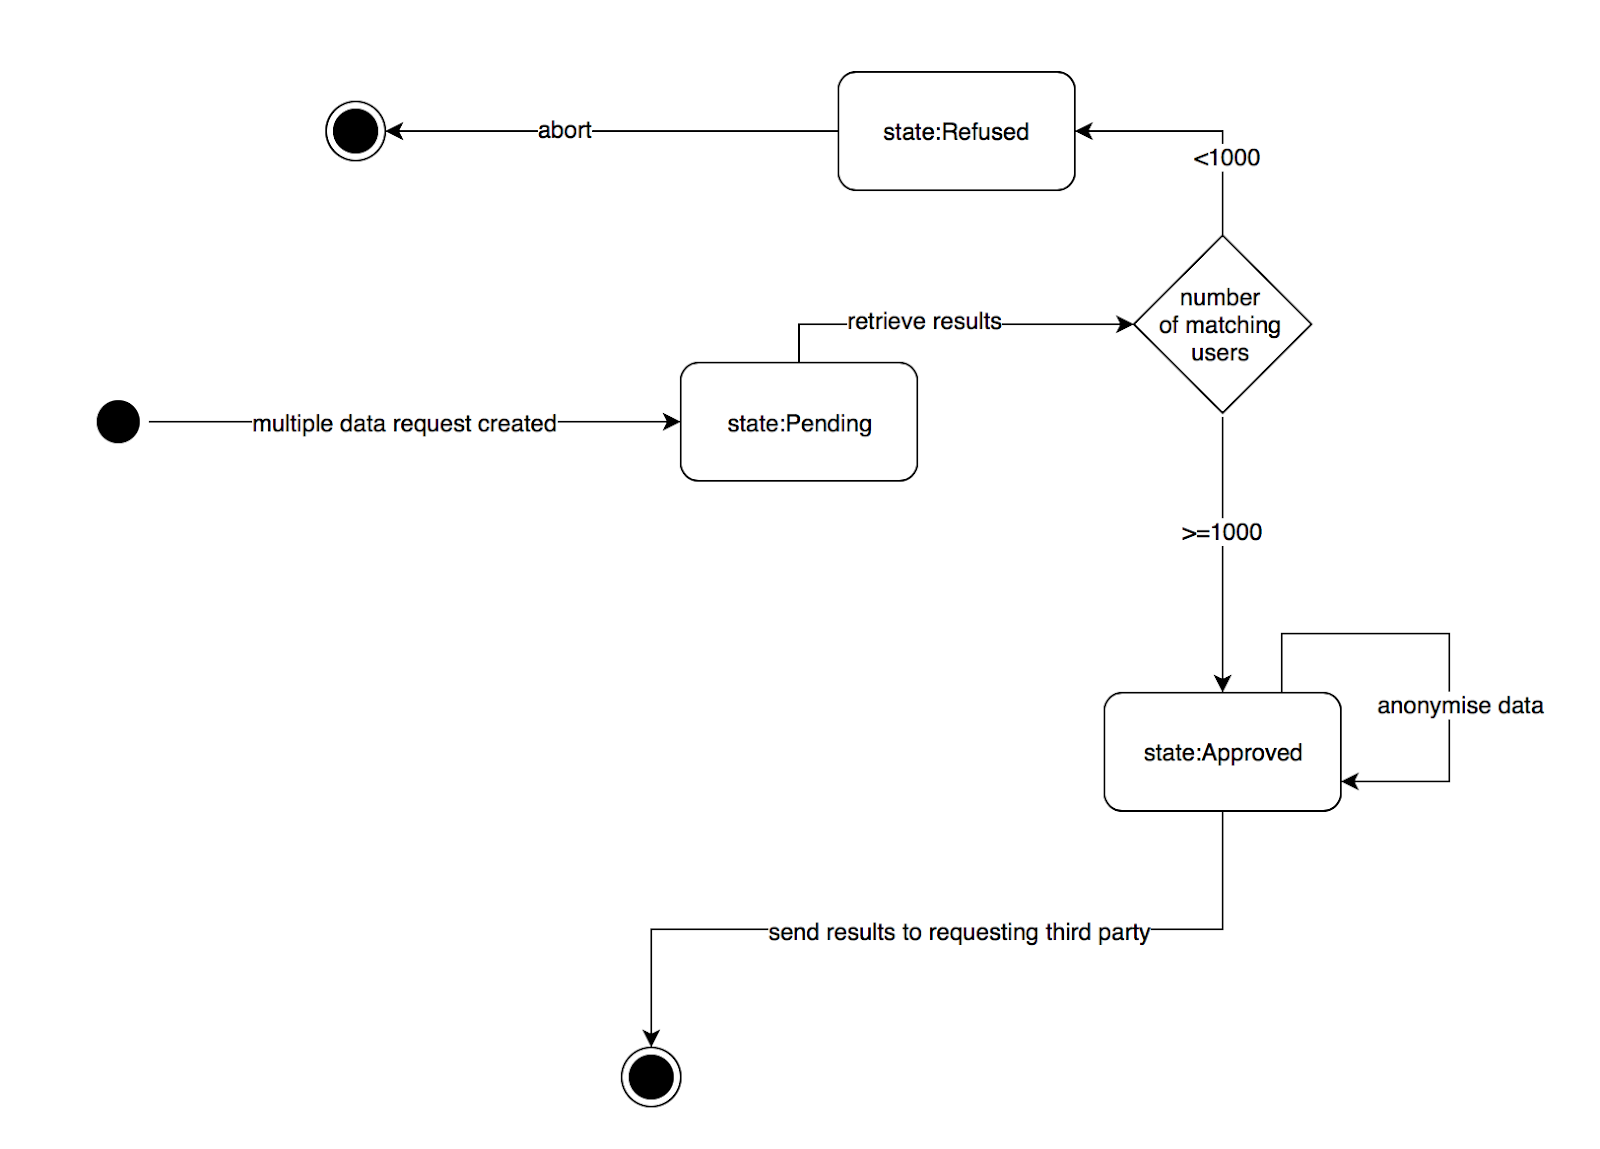
\includegraphics[width=\textwidth]{Diagrammi/groupStateChart.png}
  			\caption{ Group request state chart}
 			\label{fig:groupStateChart}
		\end{figure}
		\begin{figure}[H]
			\center
  			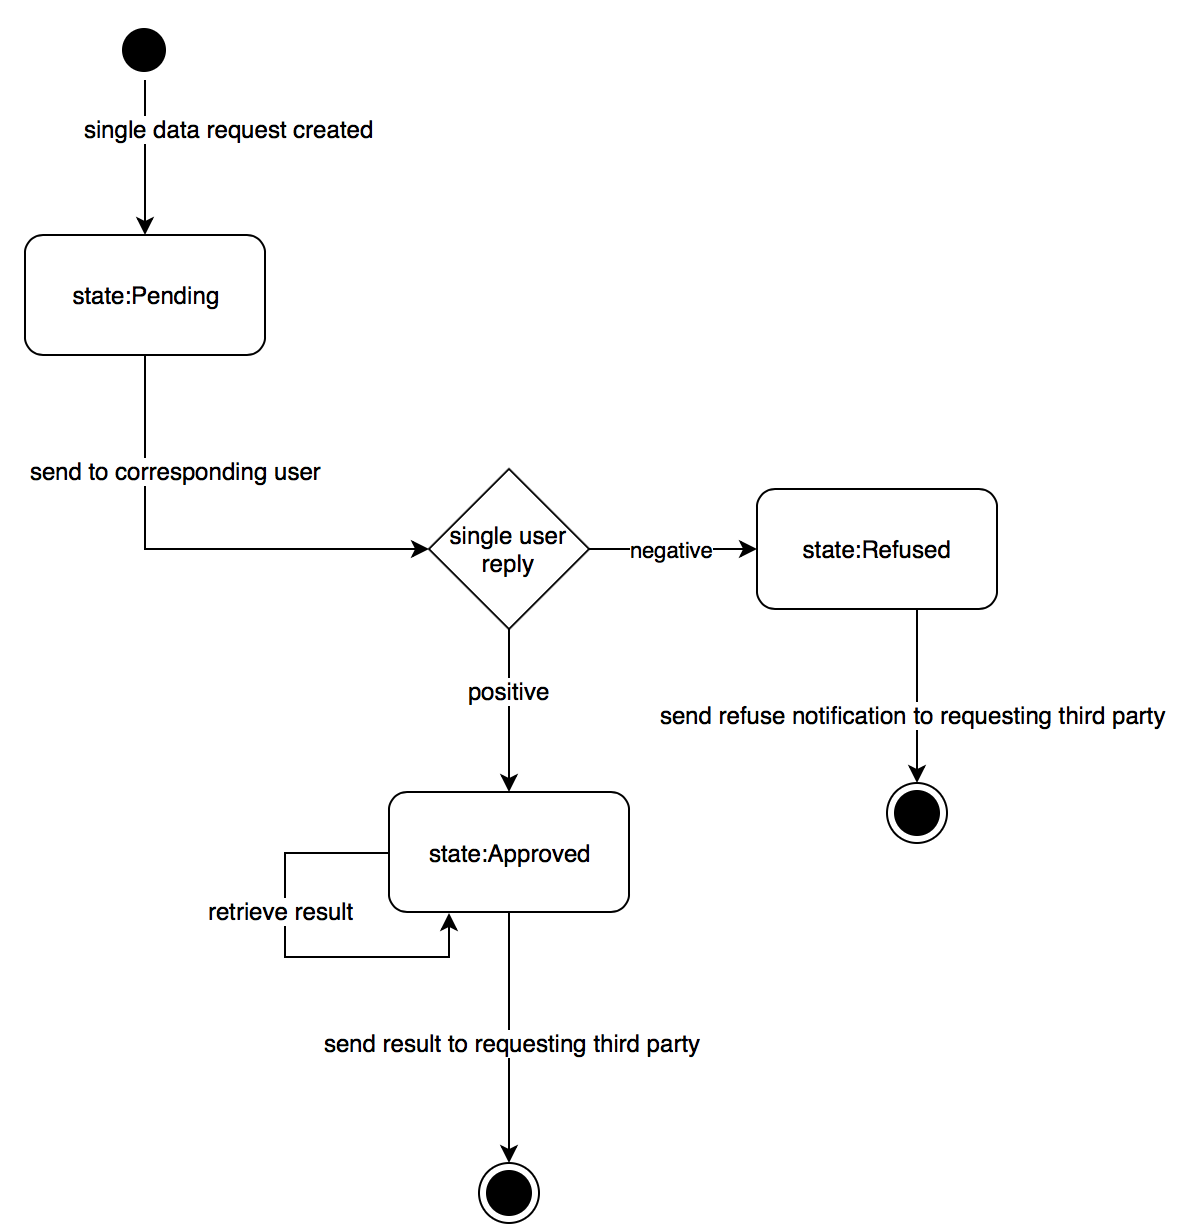
\includegraphics[width=\textwidth]{Diagrammi/singleStateChart.png}
  			\caption{ Single request state chart}
 			\label{fig:singleStateChart}
		\end{figure}

	\subsection{Product functions}
	This section is devoted to analyzing the Value Proposition that {\it Data4Help} and {\it Track4Run} provide to its users. The presented functionalities are grouped according to the user they address.\\
	
	\begin{itemize}
	\item{\bf Private User functions:}\\
	\\
	{\bf Visualize your own health status} \\
{\it Data4Help} enables {\it Single User}s to visualize their health status. This is done by retrieving all information about the user’s position and health from his device, by analyzing it and by resulting into a graphical explanation. Analysis performed on data consists of aggregations, statistical operations and derivations. Results are finally provided to the user through a clear interface containing significant plots, tables and charts.\\
Users will then refer to {\it Data4Help} to understand if they are either healthy for their age or might have some values out of range. \\

{\bf Have your health monitored} \\
{\it Data4Help} enables {\it Single User}s to have their health monitored by {\it Third Parties} by accepting their requests and allowing them to subscribe. This feature is useful especially for people having a medical condition, so that they can be remotely monitored by their doctor. Elderly people could benefit from it as well.\\

{\bf AutomatedSOS}\\
{\it AutomatedSOS} is an additional feature that, when enabled, can provide a significant help to individuals in critical situations. In fact, when the {\it System} observes some health parameters below certain thresholds an ambulance is immediately called to the user’s location. This functionality may be activated by any {\it Single User} and will function only in case of working GPS.\\

{\bf Take part in a run} \\
{\it Track4Run} gives runners, using a private account, the possibility to participate to an existing run that has not started yet. Runners will provide their data to the organizers of the run so they can be tracked on the path, allowing the {\it System} to measure key statistics such as average pace, heart rate and energy spent (if provided). This data will be shown to each runner at the end of the event, comparing him to other participants.\\

	\item{\bf Third Party functions:}\\
	\\
	{\bf Request individual’s health data}\\
A reason why {\it Third Parties} decide to register to {\it Data4Help} is to retrieve data about individuals, precisely concerning their position and their health status. {\it Data4Help} aims at allowing these companies to collect their desidered data for medical purposes. \\
The retrieval of data is possible by performing requests to {\it Single User}s, denoted with either their FC or their email. Requests contain the {\it Third Parties}’ generalities and specify whether they require the user’s data only once or want to subscribe to it, meaning that they will receive updates on the data whenever they are produced. Subscriptions must indicate a duration and can be ended by the {\it Single User} at any time. Requests may be customized by including a list of desired data types, chosen among the following:
\begin{itemize}
\item position
\item heart rate
\item activities (outdoor or indoor)
\item nutrition
\item sleep \\
\end{itemize}
Request are sent directly to the involved users and require their acceptance to proceed with the forwarding of data. Therefore a {\it Single User} can decide either to accept or reject requests of any type.\\

{\bf Perform group requests on anonymized data}\\
Another feature offered by the {\it System} to {\it Third Parties} is the possibility to perform group requests and retrieve anonymous data. The requests are received by the {\it System} and performed onto its centralized database. Researches of this type have the following features:
\begin{itemize}
\item Must concern a number of individuals greater than 1000
\item Do not include sensible data
\item Include search parameters
\item Include requested data types
\item Do not need to be accepted by users\\
\end{itemize}
If the request is valid according to the stated conditions, the {\it System} will retrieve all data matching the search parameters and present it to the requesting user. {\it Single User}s whose data is part of the query result are not involved. Therefore they neither are mentioned, in order to preserve their anonymity, nor are asked to accept or reject the request.\\

{\bf Organize new runs} \\
{\it Track4Run} gives organizers, using a {\it Third Party} account, the possibility to create a run and get data from participants. When creating a run, organizers have to define the path that the run will follow on a map, set the starting time and ending time of the event and the maximum number of participants. When a run is full no more runners can join it.\\
Throughout the event, organizers have access to live data of all participants, and can save that data after the event has finished.\\

	\item{\bf {\it Spectator} functions: }\\
	\\
	{\bf Spectate a live run} \\
	On the day of a run, any user can access {\it Track4Run} without creating any account, select a run from the list of active runs and follow it live. {\it Spectator}s can visualize the position of the users and, at the end of the run, of the final statistics of every runner.\\
During the run, {\it Spectator}s have the option to select which runner they want to track, filtering using email and FC.\\
	\end{itemize}
	
	\subsection{User characteristics}
	{\it Data4Help} addresses two types of users: {\it Single User}s and {\it Third Parties}. 
The first type corresponds to an individual of any age that downloads the application onto his device and allows access to his personal health data. In particular we have three main customer segments: elderly people, people with a medical condition and people who want to keep track of their health status. \\
The second refers to any company that provides a valid P.IVA to the {\it System}, and wants to obtain user data for medical purposes.\\
\\
{\it Track4Run}’s main targets are runners and organizers.\\
Runners, in particular, generally range from 15 to 60 years old people, of all social categories. \\
Organizers, on the other hand, must have a P.IVA, so they generally represent sport clubs or any company with medical interests.\\
When signing-up in the application, runners are forced to create a private account on {\it Data4Help}, which shares the user database with {\it Track4Run}, while organizers are forced to create a {\it Third Party} account.\\
Finally, {\it Spectator}s use the application with the sole purpose of spectating an existing run, and do not have to create an account on {\it Data4Help}.\\
\\
We will now briefly precise which types of users the {\it System} encounters at different stages:
\begin{itemize}
	\item{\it {\it Guest}: } a user who has downloaded the application onto his device, but has yet to create an account. No {\it Guest} can access the application’s functionalities prior to registration.
	\item {\it {\it Single User}: } a user who has created a “{\it Single User}” account, but has yet to log in. Once he has inserted his credentials he may access all of the application’s functionalities. 
	\item {\it {\it Third Party}: } a user who has created a “{\it Third Party}” account, but has yet to log in. Once he has inserted his credentials he may access all of the application’s functionalities.
	\item {\it Logged-in {\it Single User}: } a user that has provided the credentials to his {\it Single User} account and that may access all application functionalities.
	\item {\it Logged-in {\it Third Party}: } a user that has provided the credentials to his {\it Third Party} account and that may access all application functionalities.
	\item {\it {\it Spectator}: } a user that has not logged-in into {\it Track4Run} but is spectating an existing run. 
\end{itemize}	

	\subsection{Assumptions, dependencies and constraints}
		\subsubsection{Constraints}
		\begin{itemize}
		\item The S2B must abide to the GDPR regulation with regards to the treatment of personal data.
\item The S2B must be implemented as a smartphone application.
\item The S2B must be available in the Italian application stores only (based on the OS).

		\end{itemize}
		\subsubsection{Dependencies}
		\begin{itemize}
		\item The S2B will make use of the GPS services offered by users’ smartphones.
\item The S2B will access the APIs provided by health monitoring applications integrated by default in the smartphones.
\item The S2B will access the necessary APIs to make phone calls on behalf of the user.
\item The S2B will make use of internet access provided by users’ smartphones. 
\item The S2B will make use of a map visualization service.
\item The S2B will make use of a {\it Third Party} storage {\it System}.
		\end{itemize}
		
		\subsubsection{Domain Assumptions}
		\begin{itemize}
		 \item {\bf [D1]}  Each user will create only one account.				
			 \item {\bf [D2]} The FC and email provided during registration are valid and belong to the person who’s creating the account..
   			 \item {\bf [D3]} The P.IVA of a {\it Third Party} is valid and specific to that company.
   			 \item {\bf [D4]}  Data provided to the {\it System} is related to the person whose account was used to provide it.
   			 \item {\bf [D5]} All health data directly provided by the user represents his real health status.
			  \item {\bf [D6]}  Position data has an accuracy of 10 meters around the actual position.				
			 \item {\bf [D7]} Health data has a relative error lower than 5\%.
   			 \item {\bf [D8]} Permission to access health and GPS data is always granted to the S2B.
   			 \item {\bf [D9]} {\it Third Parties}, including organizers, collect data only for medical purposes.
   			 \item {\bf [D10]} Data is stored on persistent memory.
			 \item {\bf [D11]} The storage {\it System} is fully replicated and fault-tolerant, so that a copy of a specific piece of data is always available.			
			 \item {\bf [D12]} Permission to make calls is always granted to the S2B.   			 
			 \item {\bf [D13]} Users’ smartphones always have signal when needed by {\it AutomatedSOS}.
   			 \item {\bf [D14]} Users’ smartphones always have internet access when the S2B needs it.
   			 \item {\bf [D15]} The path specified when creating a run is feasible. \\
		\end{itemize}
		{\bf[D10]} and {\bf [D11]} are crucial since the S2B will make use of a {\it Third Party}’s Database, and thus can’t enforce its reliability.\\
{\bf [D12]} and {\bf [D13]} are needed to ensure the nonfunctional requirements of {\it AutomatedSOS}, otherwise the S2B should keep trying to reach an emergency number until it’s successful.\\
{\bf [D14]} is a strong assumption, generally the mobile application could keep pinging the server until the connection is established again.\\

\pagebreak	

%Specific Requirements
\section{Specific Requirements}
	
	\subsection{External Interface Requirements}
		
		\subsubsection{User Interfaces}
		\begin{itemize}
			\item {\bf DATA4HELP INTERFACES} 
			\begin{itemize}

				\item{\bf Logo}\\
			{\it Data4Help}’s Logo represents a heart containing the sketch of a pulse. This simple image fully captures the purpose of the service: to collect data concerning individuals’ health and allowing it to be monitored. \\
The logo is also used as the application’s icon and will be visible to whoever downloads the app onto his device.
					\begin{figure}[H]
						\center
  						
\includegraphics[width=0.7\columnwidth]{D4HLogo.jpg}
  						\caption{{\it Data4Help} Logo}
 						\label{fig:Logo}
					\end{figure}

				\item{\bf Login or Signup}\\
			When a {\it Guest} downloads {\it Data4Help} for the first time, the first interface will ask the user to choose between login and signup. If the user has already created an account he will choose to login in order to access the application’s functionalities. If the user instead has not created an account yet he will choose the signup option.\\
					\begin{figure}[H]
						\center
  						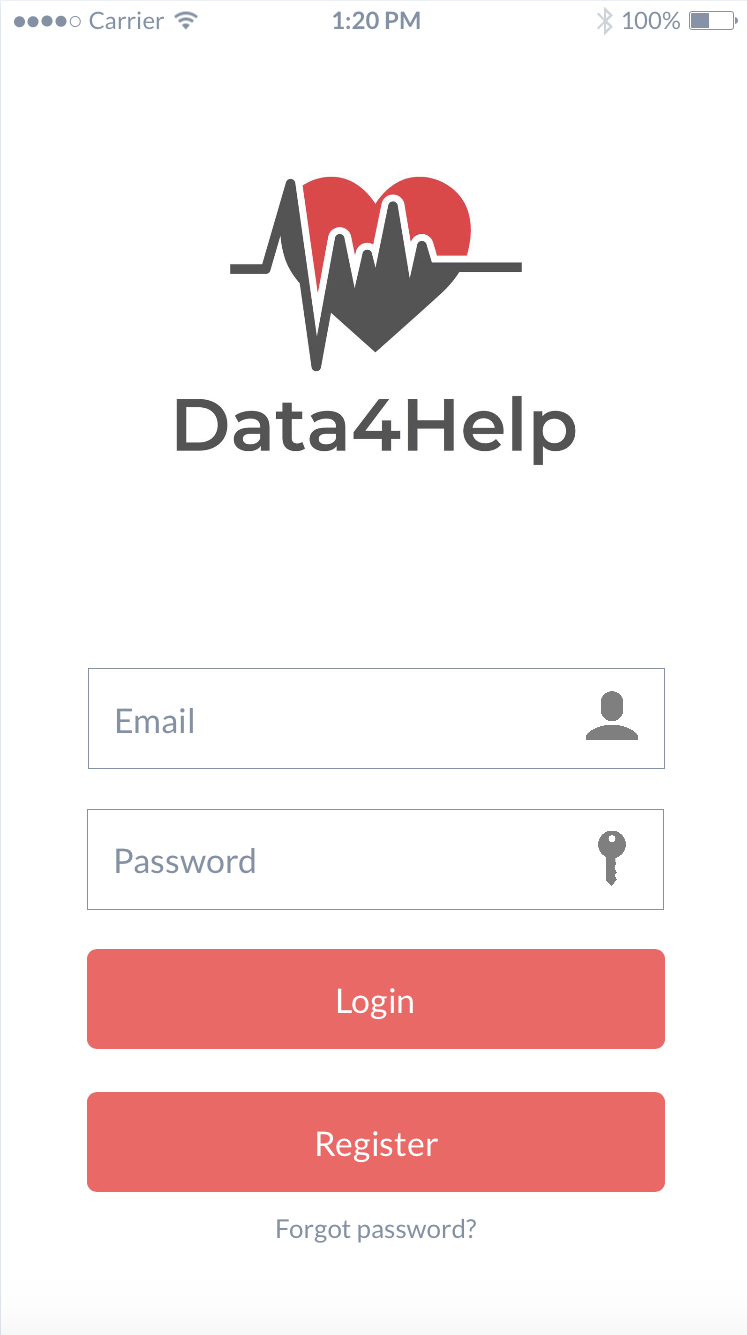
\includegraphics[width=5cm]{Mockup/mockupLogin.png}
  						\caption{Login interface}
 						 \label{fig:Login}
					\end{figure}

				\item{\bf Tutorial}\\
				When a {\it Guest} decides to create a new account {\it Data4Help} provides him with a simple guide to the service. The user will easily swipe from one page to another and follow the tutorial on all the features it can access after registration. \\
					\begin{figure}[H]
						\center
  						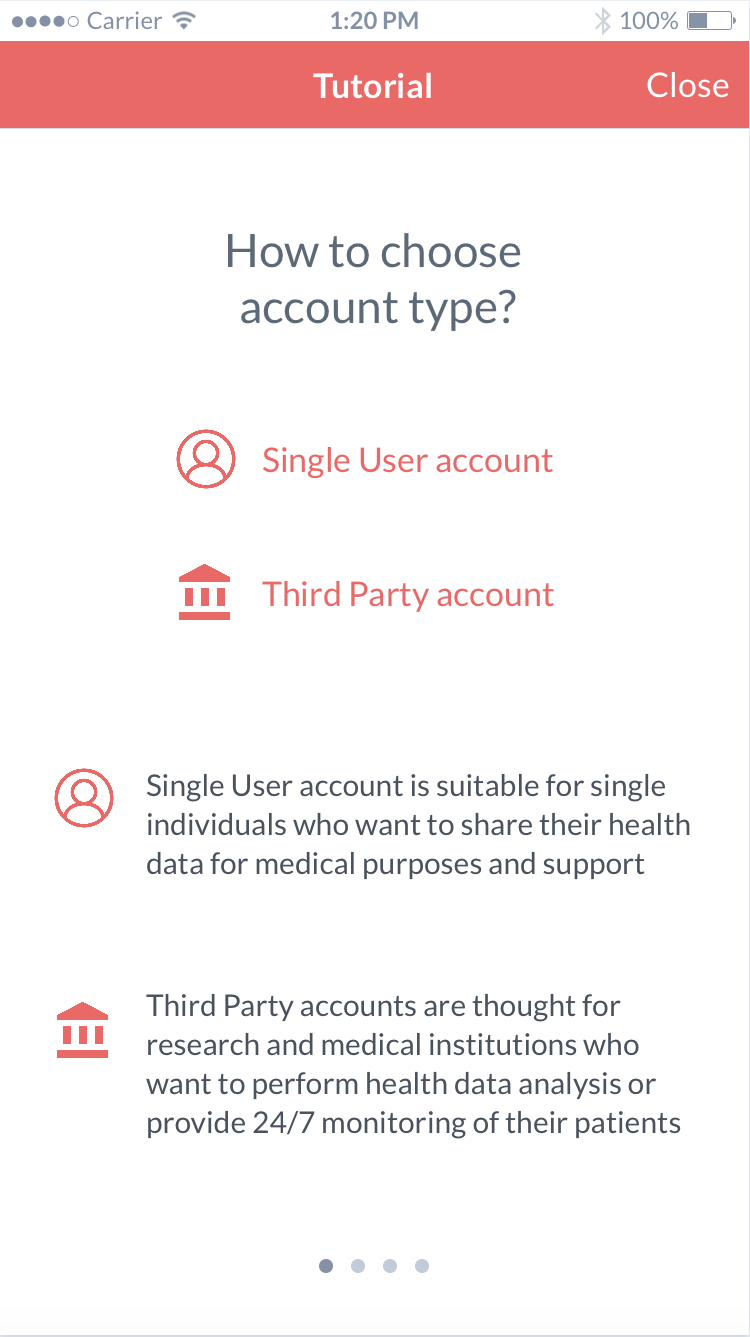
\includegraphics[width=5cm]{Mockup/mockupTutorial.png}
  						\caption{Tutorial interface}
 					 	\label{fig:Tutorial}
					\end{figure}

				\item{\bf Create an account}\\
				Following the initial guide a {\it Guest} will be able to create an account and register to the service. The user will be asked to select which type of account to create: {\it Single User} or {\it Third Party}. Once the type has been selected, the user will be asked to fill in a form with his general information, an email that will identify him uniquely and a password. Furthermore, according to the type of account, a user will have to provide a unique FC or P.IVA if creating respectively a {\it Single User} account or {\it Third Party} account.\\
				
\begin{figure}[H]%
    \centering
    \subfloat[{\it Single User} registration interface]{{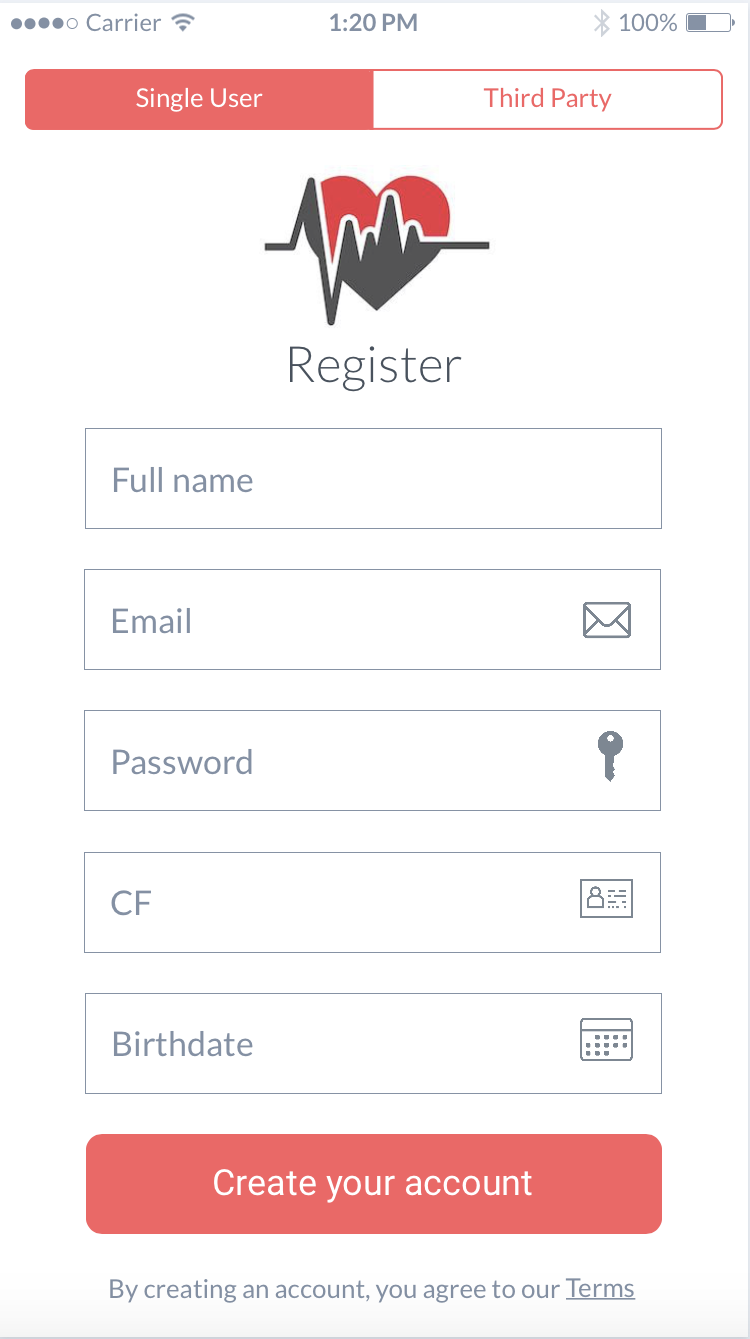
\includegraphics[width=5cm]{Mockup/mockupRegisterSU.png} }}%
    \qquad
    \subfloat[{\it Third Party} registration interface]{{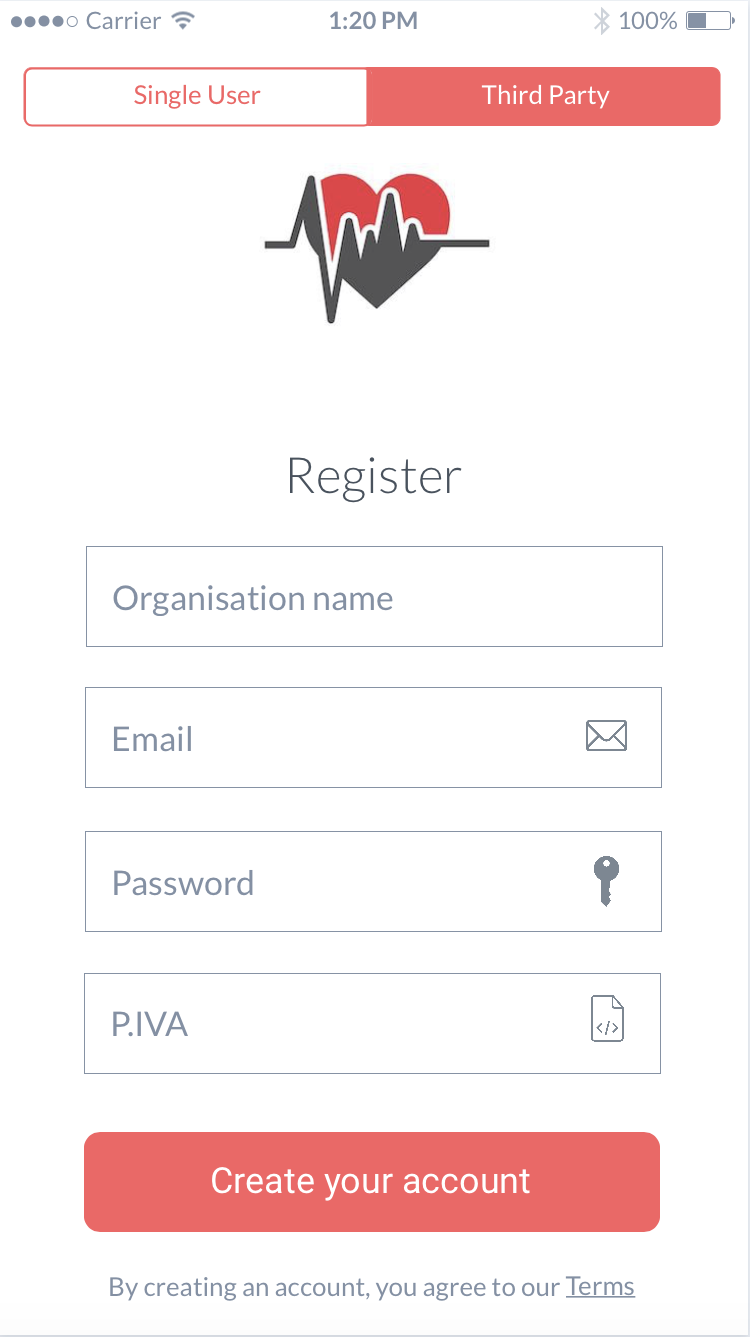
\includegraphics[width=5cm]{Mockup/mockupRegisterTP.png} }}%
    \caption{Create an account}%
    \label{fig:CreateAccount}%
\end{figure}

				\item{\bf Single User Interface} \\
			When a user signs in with a {\it Single User} account he is presented with the first of a sequence of interfaces, all handled by a Tab Bar Controller. We will now detail the features of each tab:
				\begin{itemize}
					\item[$\circ$] {\bf My Health tab} \\
				My Health tab is the default tab, the first interface presented to the {\it Single User}. It displays a summary of the user’s health, measured thanks to the data imported from the device onto which the app is downloaded. This is the interface that a user will access in order to monitor his health status and have a clear view of how his parameters compare to the average for his age. Furthermore, plots, tables and charts will guarantee a more user friendly experience.\\
Finally in this section the user will be able to activate at anytime {\it AutomatedSOS}. A simple click on the SOS icon will enable this feature and immediately contact an ambulance in case of critical health status.\\
					\begin{figure}[H]
						\center
  						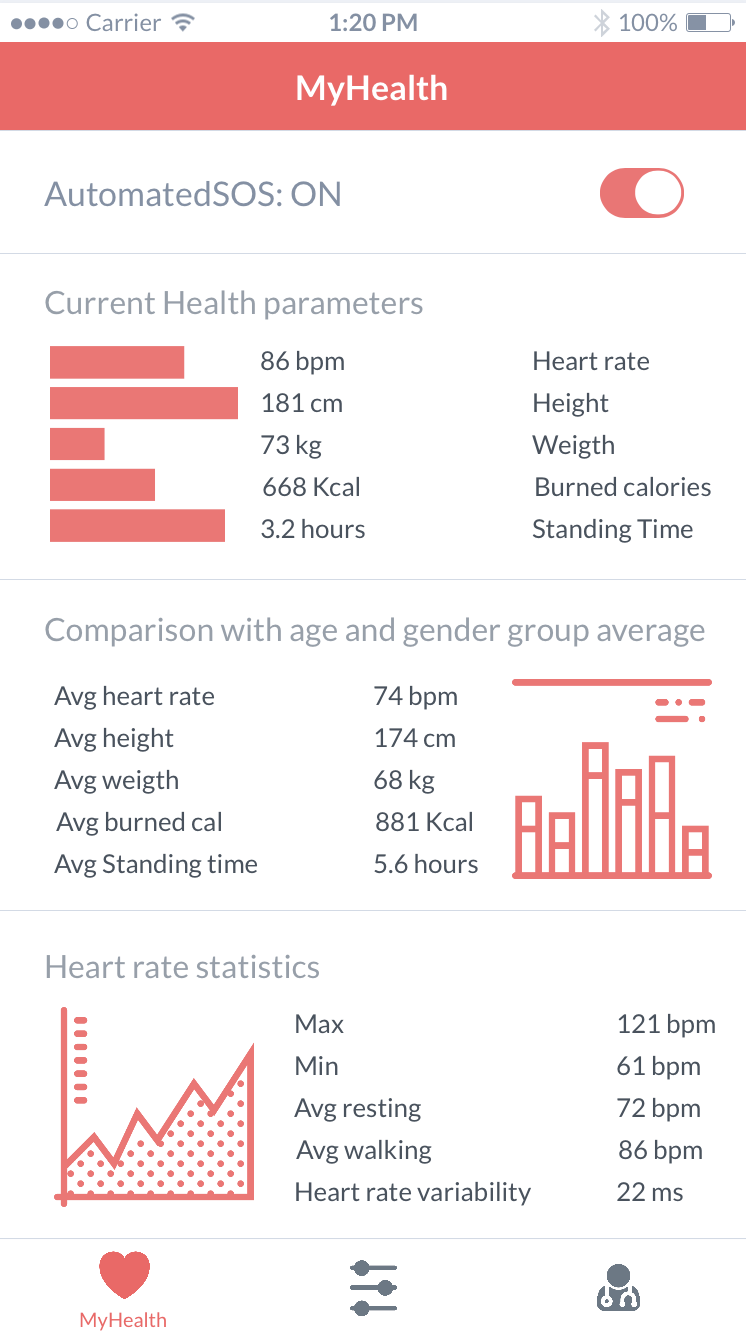
\includegraphics[width=5cm]{Mockup/mockupMyHealth.png}
  						\caption{My Health tab}
 					 	\label{fig:MyH}
					\end{figure}

					\item[$\circ$] {\bf My Settings tab}  \\
				My settings is the tab that allows a user to manage his personal data associated to his account. In this section a user may at any time modify his general information and password. However a user can never change the email and CF associated to its account as they are its unique identifiers.\\
In this screen the user will find all the information linked to its account in a list, where each item can be modified at any time. After any modification the user will have to save its updates in order to notify the application’s server.\\
					\begin{figure}[H]
						\center
  						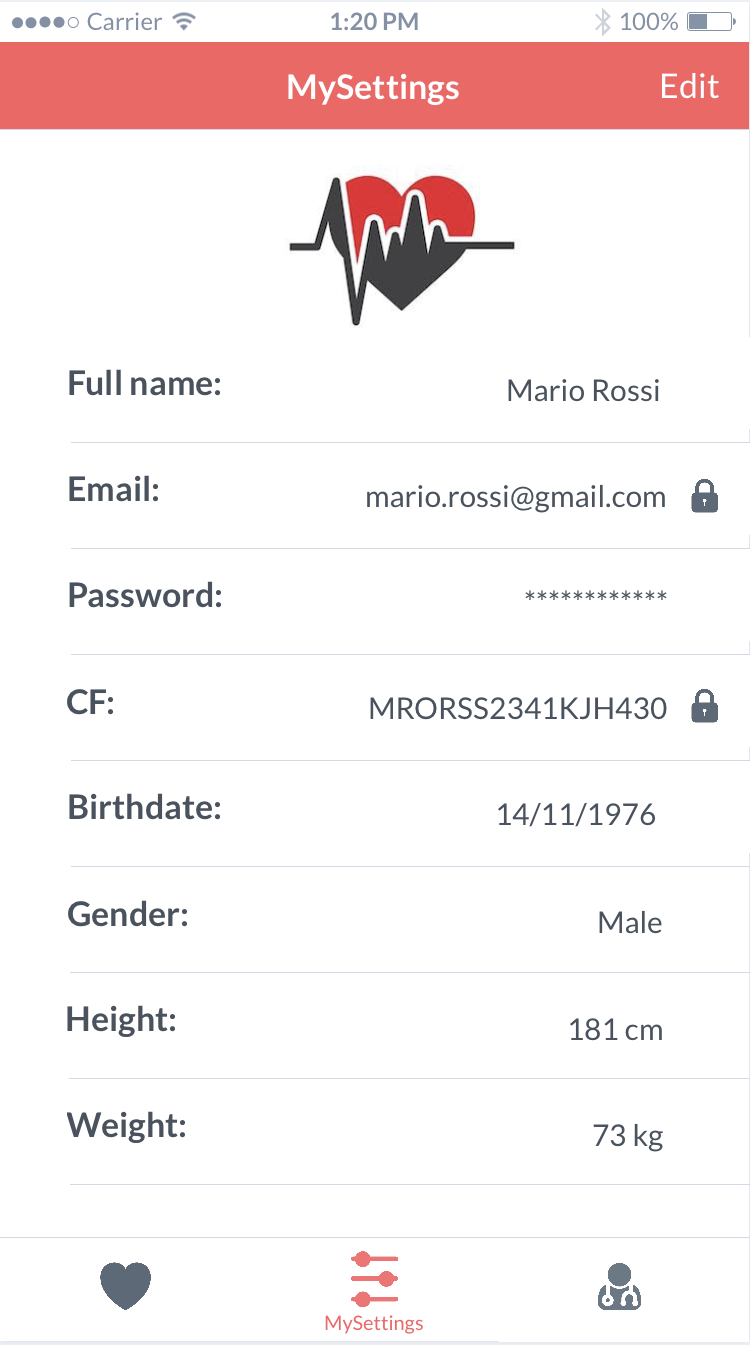
\includegraphics[width=5cm]{Mockup/mockupSettingsSU.png}
  						\caption{My Settings tab}
 					 	\label{fig:MyS}
					\end{figure}

					\item[$\circ$] {\bf My Followers tab}  \\
				My followers is the tab that allows a user to keep track of all the {\it Third Parties} requesting his data. These include both those {\it Third Parties} that have performed single requests and those that have subscribed to the user’s data. Furthermore in this section the user will also be able to accept or reject pending requests.\\
					\begin{figure}[H]
						\center
  						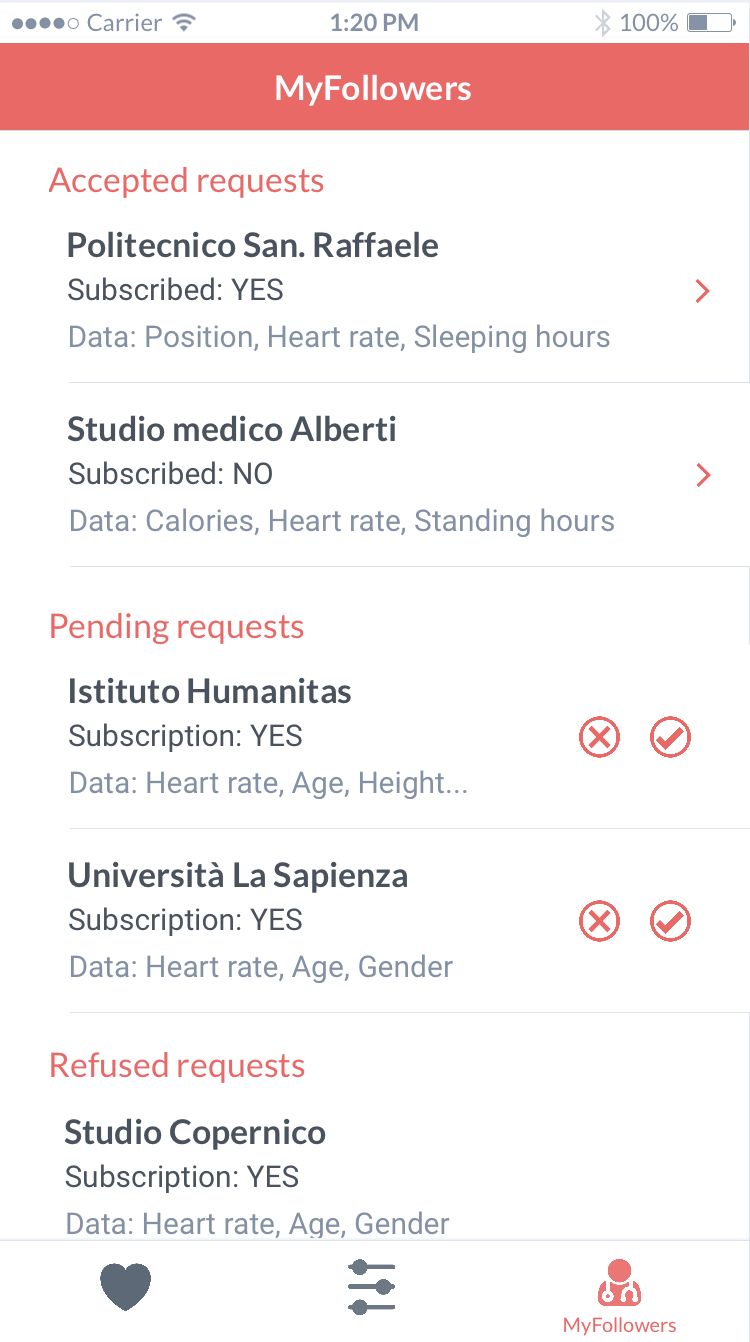
\includegraphics[width=5cm]{Mockup/mockupMyFollowers.png}
  						\caption{My Followers tab}
 					 	\label{fig:MyF}
					\end{figure}

				\end{itemize}
			
				\item{\bf Third Party Interface}
				\begin{itemize}

					\item[$\circ$] {\bf Research tab} \\
				The research tab is the default tab, the first interface presented to the {\it Third Party}. This is the section in which the {\it Third Party} can perform requests to individuals or on groups of users. The interface suggests the user to select one of the two types of requests. According to the selected type, the {\it Third Party} will have to fill in a form providing all the necessary parameters to perform the research.\\
				
\begin{figure}[H]%
    \centering
    \subfloat[Single Request ]{{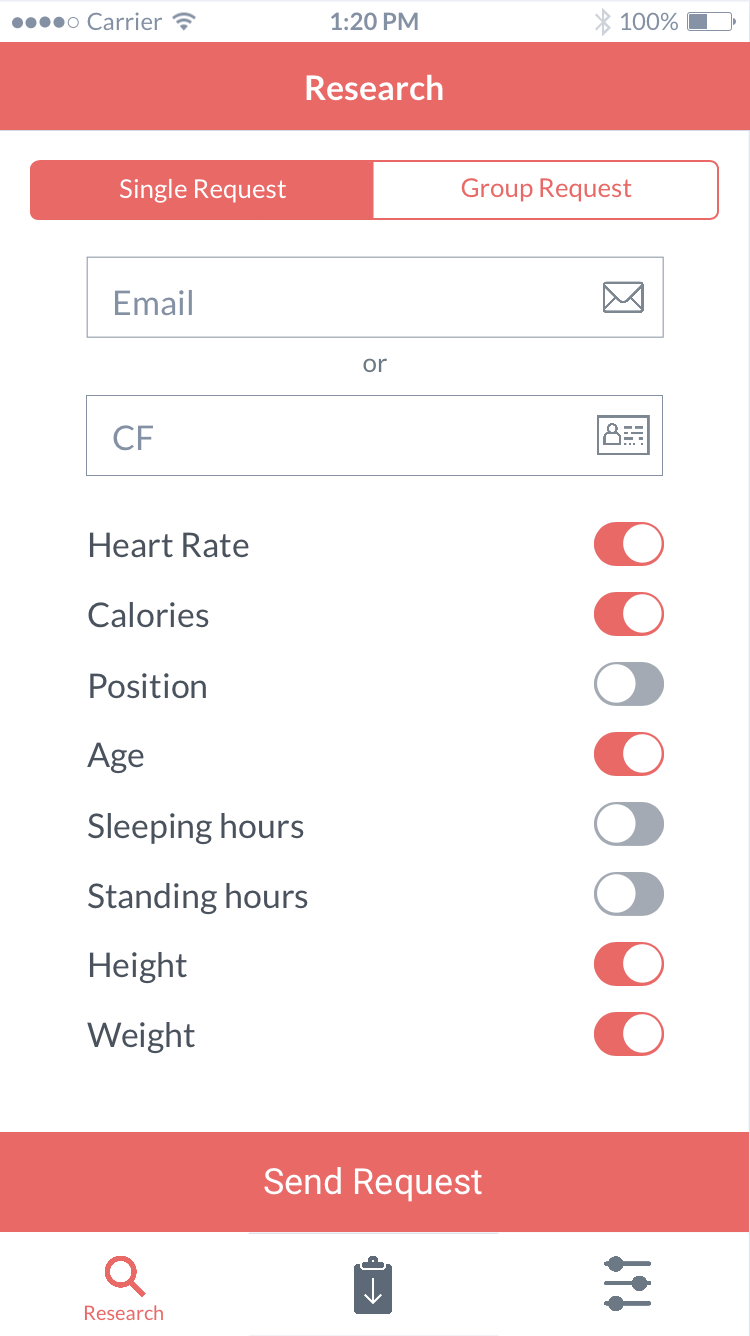
\includegraphics[width=5cm]{Mockup/mockupSingleRequest.png} }}%
    \qquad
    \subfloat[Group Request ]{{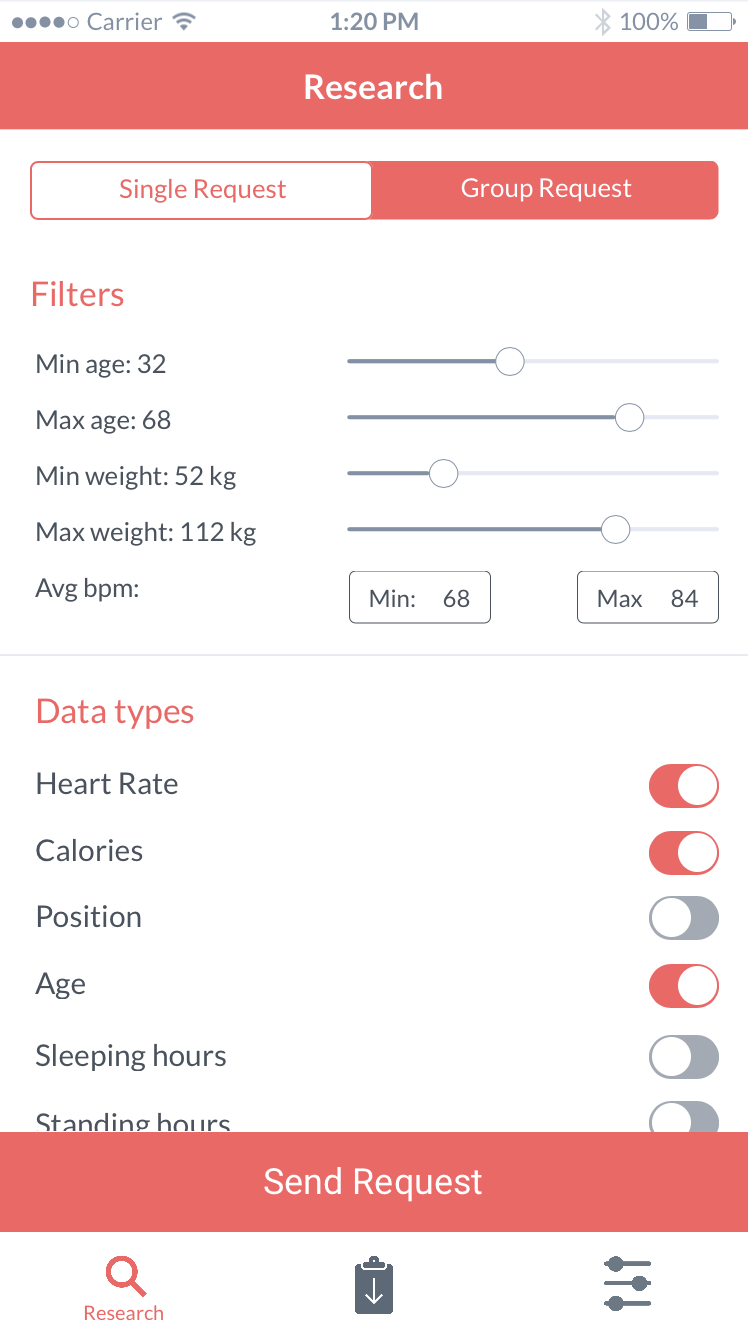
\includegraphics[width=5cm]{Mockup/mockupGroupRequest.png} }}%
    \caption{Research tab}%
    \label{fig:RequestTab}%
\end{figure}

					\item[$\circ$] {\bf History tab}\\
				In this tab the {\it Third Party} will be able to save all the searches it has performed on individuals or anonymous groups of users. The screen displays a list of items in chronological order, each representing an old or pending request.\\
Each item in the list has the following features:
						\begin{itemize}
							\item name: FC or email of an individual, in case of a single request, or brief description of the group of users, in case of a group request.
							\item download button: enables the {\it Third Party} to download at any time the CSV file containing the requested data, or to have it sent by email.
							\item subscription button: allows at any time to end a subscription to a certain request. In case of single requests, the subscription will be active only if the user grants his permission with a positive response.\\
					\begin{figure}[H]
						\center
  						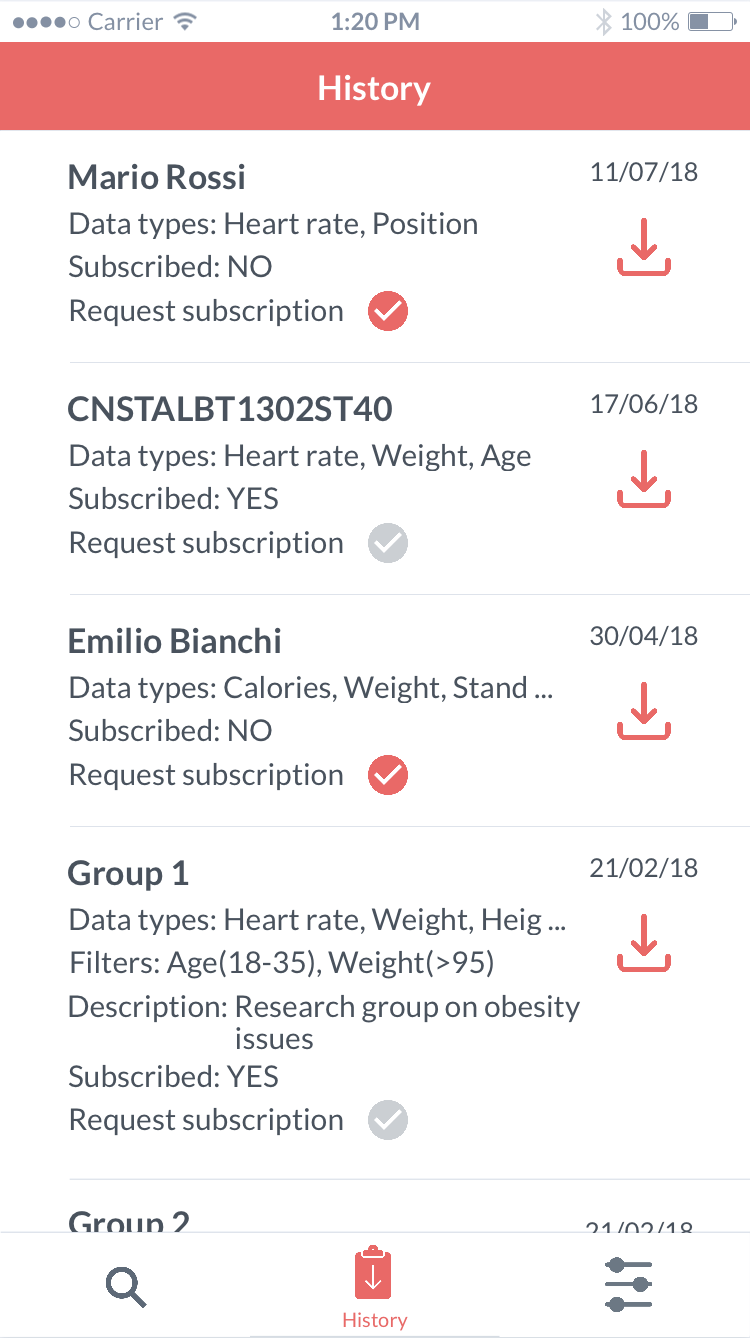
\includegraphics[width=5cm]{Mockup/mockupHistory.png}
  						\caption{History tab}
 					 	\label{fig:Hist}
					\end{figure}
						\end{itemize}
						

					\item[$\circ$] {\bf My Settings tab}  \\
				In this section the {\it Third Party} is able to manage its general information associated to its account and possibly modify its password. However a {\it Third Party} cannot change the email and P.IVA uniquely linked to its account as they are its unique identifiers.\\
In this screen the user will find all the information linked to its account in a list, where each item can be modified at any time. After any modification the user will have to save its updates in order to notify the application’s server.\\
					\begin{figure}[H]
						\center
  						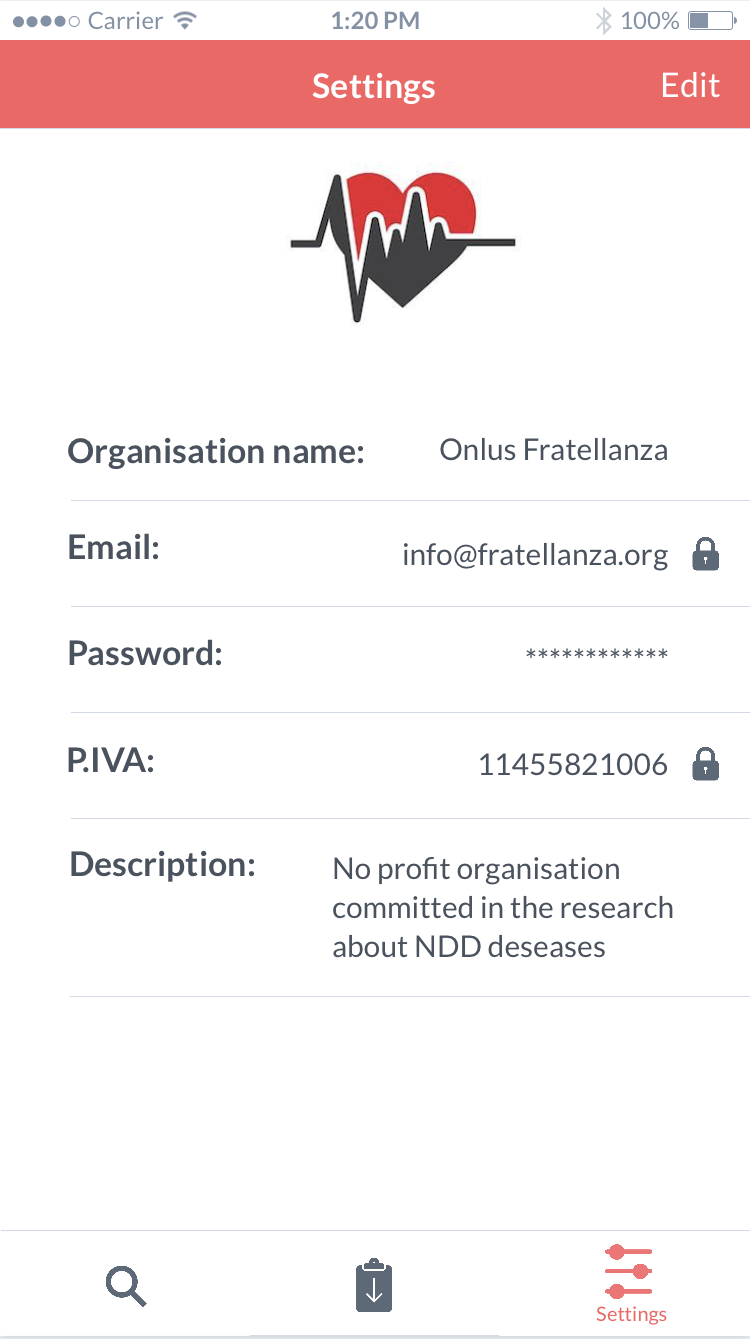
\includegraphics[width=5cm]{Mockup/mockupSettingsTP.png}
  						\caption{My Settings tab}
 					 	\label{fig:MySTP}
					\end{figure}

				\end{itemize}
			\end{itemize}
			\item {\bf TRACK4RUN INTERFACES} 	
			\begin{itemize}
				\item{\bf Logo}\\
			While reminiscing its underlying service’s logo with the sketch of a heart pulse, {\it Track4Run}’s logo is iconic on its own. The image stands out for its simple but direct meaning. The symbols of a runner and the heart pulse in a red colored background immediately convey the purpose of the application: to track runners during their activity while keeping track of their health.\\
The logo is also used as the application’s icon and will be visible to whoever downloads the app onto his device.

					\begin{figure}[H]
						\center
  						
\includegraphics[width=0.7\columnwidth]{T4RLogo.jpg}
  						\caption{{\it Track4Run} Logo}
 						\label{fig:Loogo}
					\end{figure}
				\item{\bf Login, Signup or access as {\it Spectator}}\\
				Whenever a user downloads {\it Track4Run} for the first time, he will be immediately asked to login, sign up or access as a {\it Spectator}. A user can only login with his {\it Data4Help} account. If absent, he may create it at the moment and can therefore access all {\it Data4Help}’s services through its exclusive app. However, even without an account, a user will still be able to access one of {\it Track4Run}’s services, that look for an active run a follow its participants live on the track.\\
		

				\item{\bf Single User Interfaces}
			When a user logs into {\it Track4Run} as a {\it Single User} he will be able to access all different features through a tab bar controller. We shall now start describing each tab’s purpose:
				\begin{itemize}
					\item[$\circ$] {\bf My Run tab} \\
					The MyRun tab is the default interface, showed as soon as a user logs into his account. In this section a user can see the active run he has decided to join, check its starting and ending time and its path on a map.\\
					\begin{figure}[H]
						\center
  						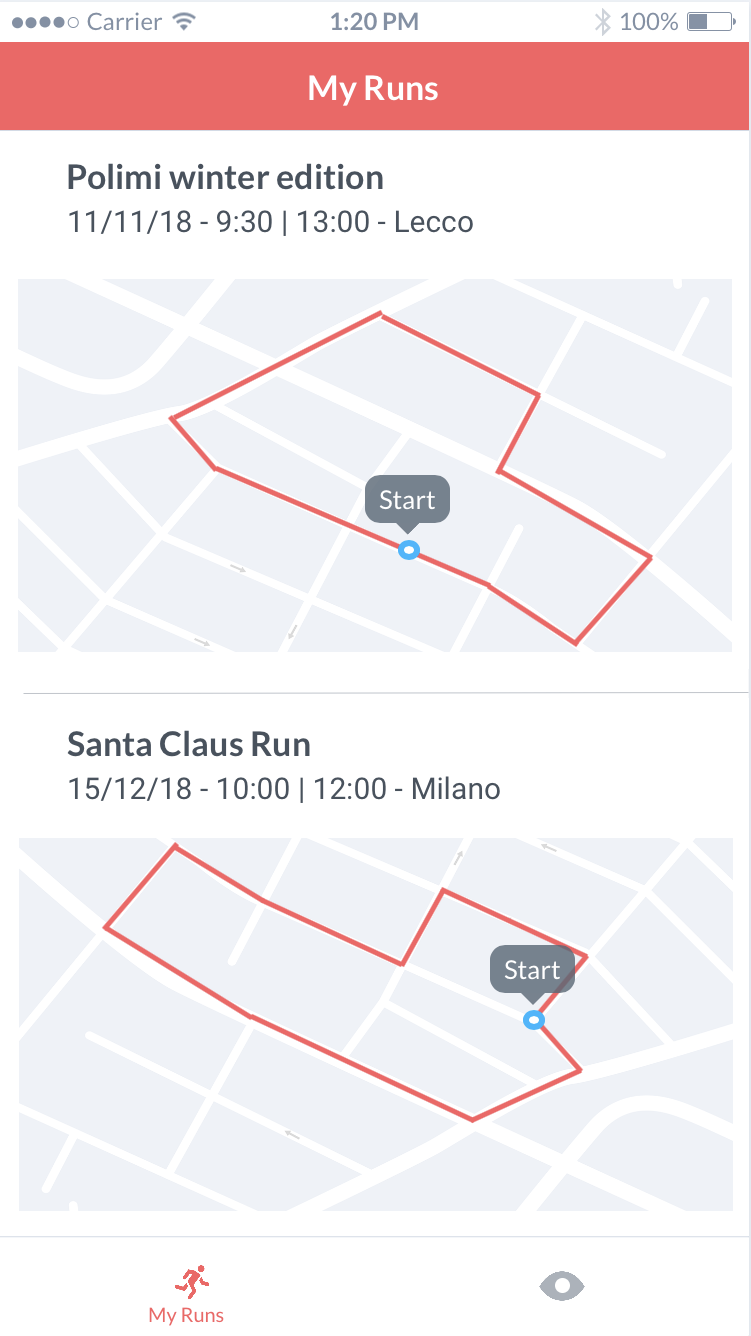
\includegraphics[width=5cm]{Mockup/mockupMyRunSU.png}
  						\caption{My run tab}
 					 	\label{fig:MyRun}
					\end{figure}

					\item[$\circ$] {\bf Active Runs tab} \\
Active Runs tab is an interface in which a user can scroll through a list of all active runs and decide whether to monitor it as a {\it Spectator} or to join it. When looking for a specific run, a user can either run through the entire list or research it by its unique identifier. Furthermore a user may also want to filter the list by location, in order to find the closest runs to his position.\\
					\begin{figure}[H]
						\center
  						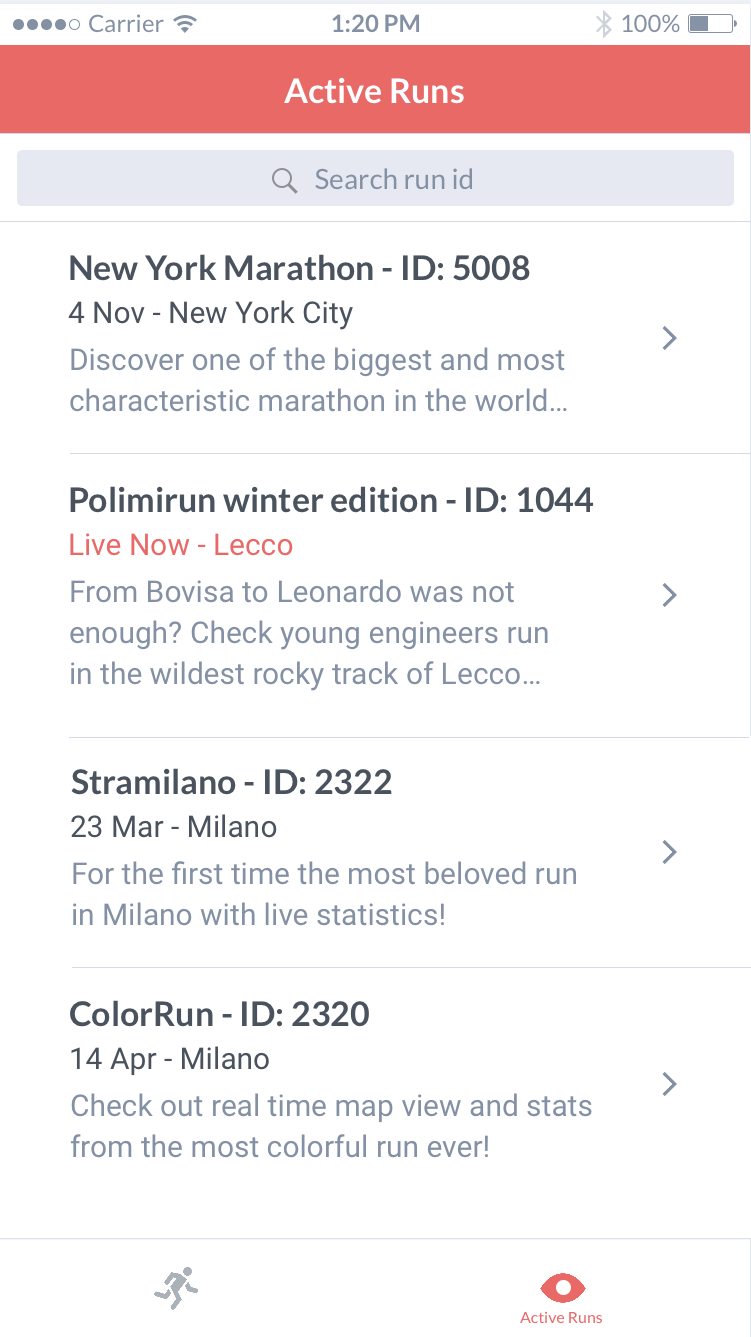
\includegraphics[width=5cm]{Mockup/mockupActiveRunsSU.png}
  						\caption{Active runs tab}
 					 	\label{fig:ActiveRuns}
					\end{figure}
				\end{itemize}

				\item{\bf Third Party Interfaces} 
			Also {\it Third Parties} will access all {\it Track4Run}’s features by navigating through a tab bar controller. We shall briefly describe each tab’s features:
				\begin{itemize}
					\item[$\circ$] {\bf New Run tab} \\
					New Run tab is the default tab in a {\it Third Party}’s interface. In this section a {\it Third Party} can organize a new run. A form where to fill in the run’s detail is immediately presented to the user. In order to create a new run the user will have to provide a name for it, a starting and ending time and finally will have to select the desired path onto a map. After having submitted the new run, the {\it Third Party} will receive the run’s unique identifier and the newly created will appear in the My Runs tab.\\
					\begin{figure}[H]
						\center
  						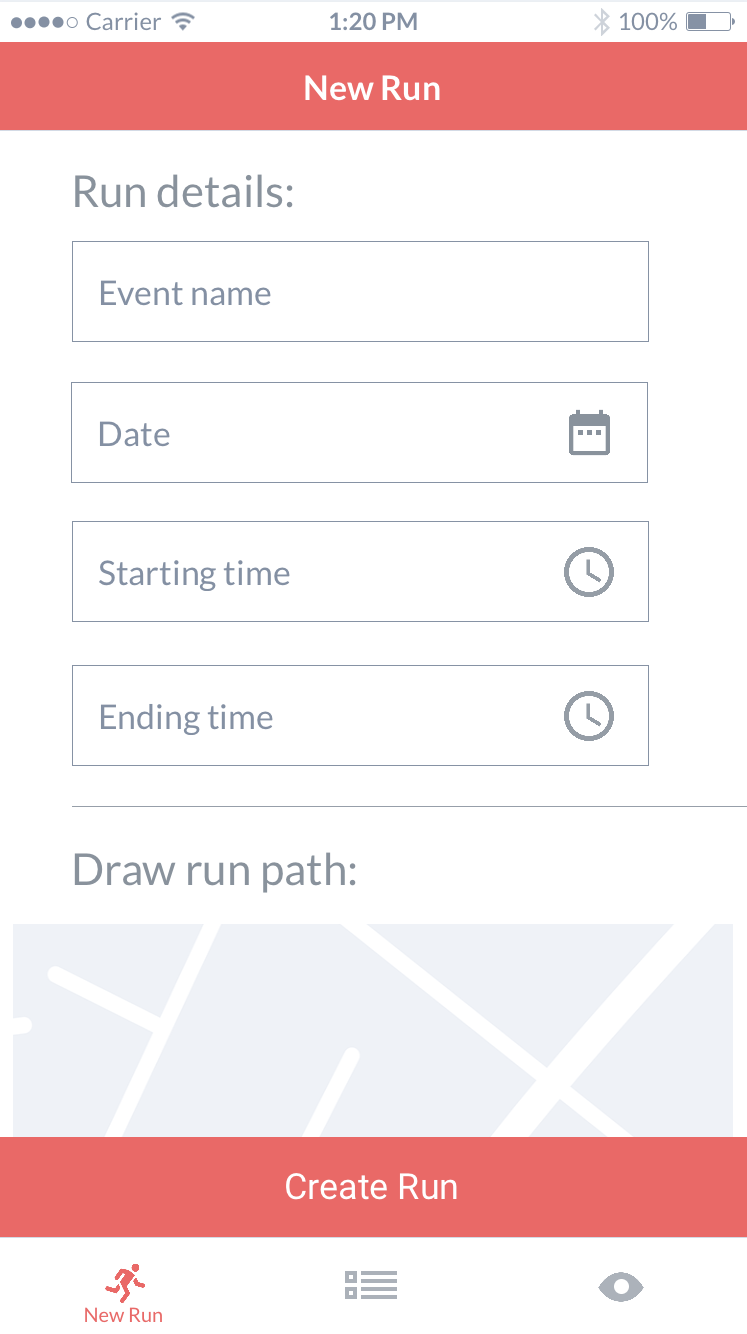
\includegraphics[width=5cm]{Mockup/mockupNewRun.png}
  						\caption{New run tab}
 					 	\label{fig:NewRun}
					\end{figure}

					\item[$\circ$] {\bf My Runs tab} \\
					This section keeps a history of all runs a {\it Third Party} has organised, both past and active ones. As soon as {\it Third Party} creates a new run this will immediately appear on top of the list. For all runs, the organiser will be able to see who has participated or will participate to it and will be able to download a file containing all the runners’ health data. The types of downloaded data will depend on those accepted to be shared by each participant. \\
					\begin{figure}[H]
						\center
  						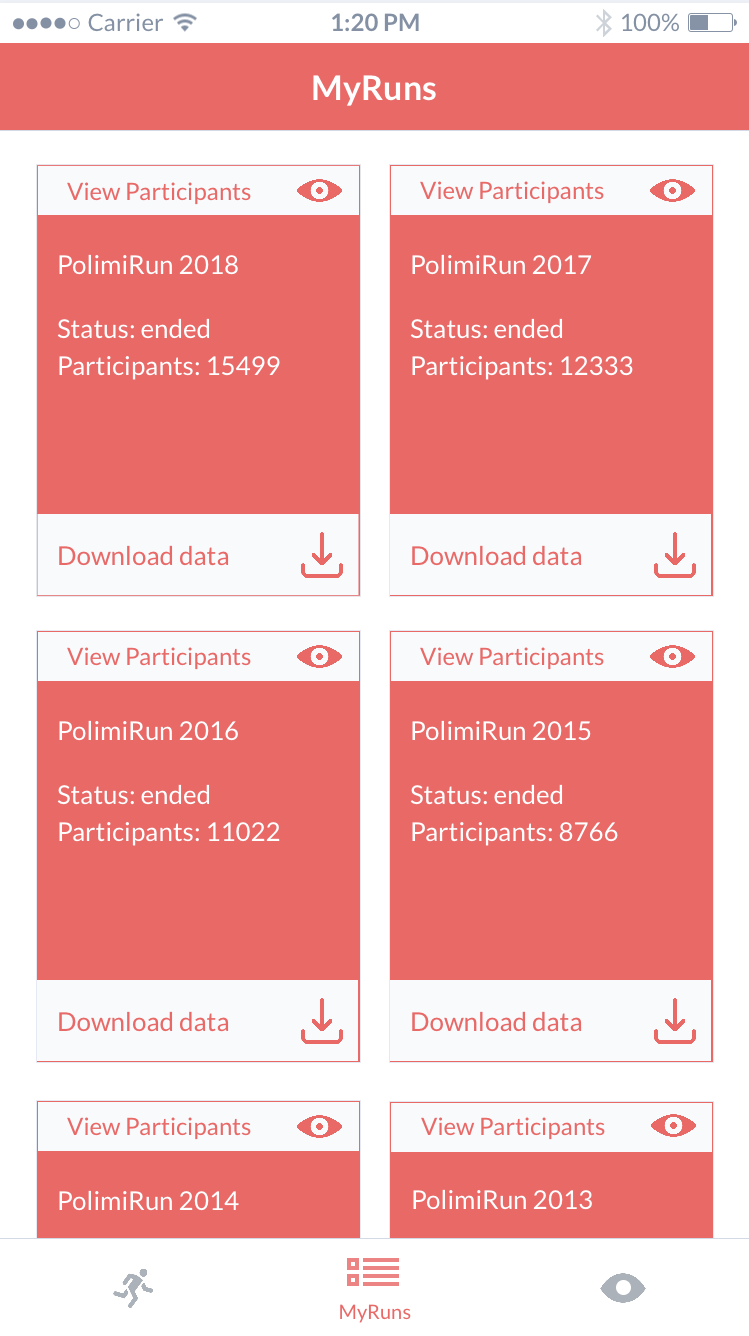
\includegraphics[width=5cm]{Mockup/mockupMyRuns.png}
  						\caption{My runs tab}
 					 	\label{fig:MyRuns}
					\end{figure}

					\item[$\circ$] {\bf Active Runs tab} \\
					In this section a {\it Third Party} can check all active runs at the moment and will be able to monitor one as a {\it Spectator}. To look for a specific run the user can either scroll through the entire list or enter a specific run’s ID. Furthermore the user can also filter the list my entering a location.\\
					\begin{figure}[H]
						\center
  						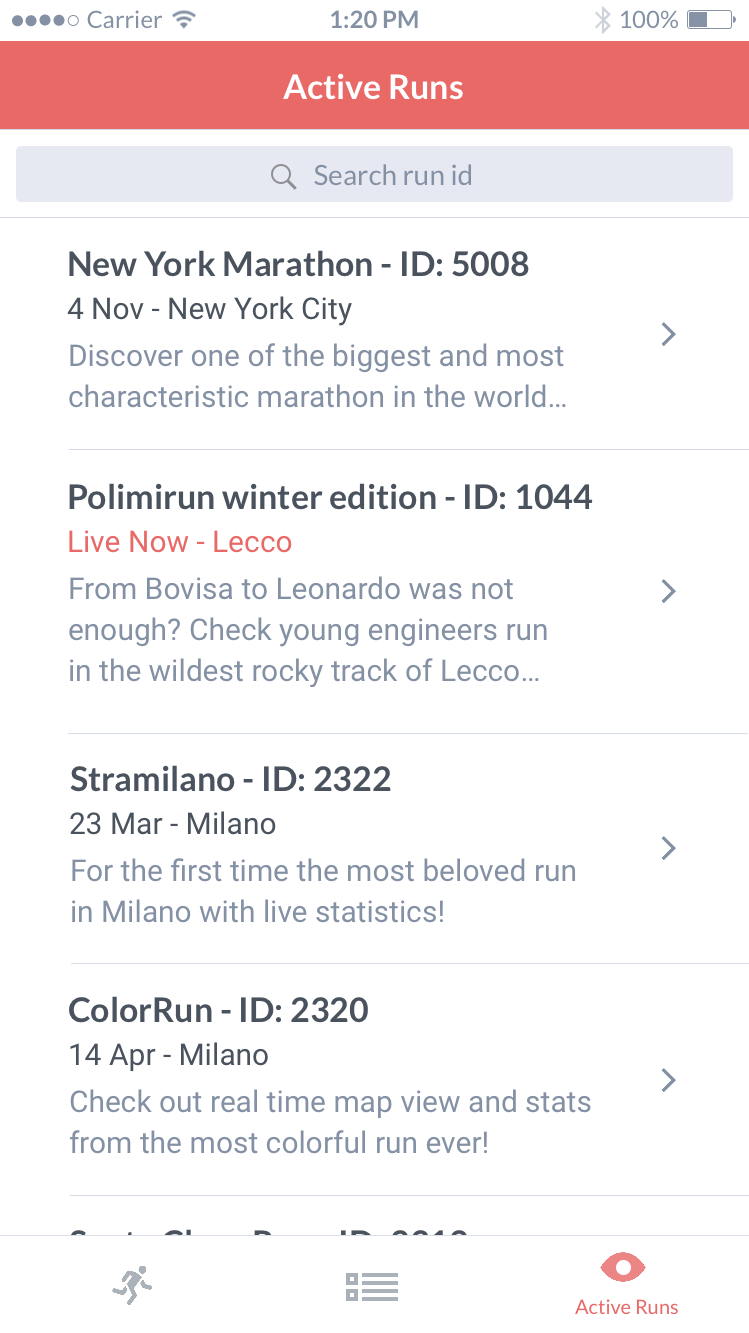
\includegraphics[width=5cm]{Mockup/mockupActiveRuns.png}
  						\caption{Active runs tab}
 					 	\label{fig:Active runs}
					\end{figure}

				\end{itemize}
				\item{\bf {\it Spectator} Interfaces} 
				\begin{itemize}
					\item[$\circ$] {\bf Research by identifier or in a list} \\
					Whenever a user access the application as a {\it Spectator}, that is without logging in, he will be presented with a unique interface with a list of all active runs. The user can scroll through the entire list of active runs and select one to spectate. Furthermore a run can be researched by entering its unique ID or by filtering the list with a location.\\
					\begin{figure}[H]
						\center
  						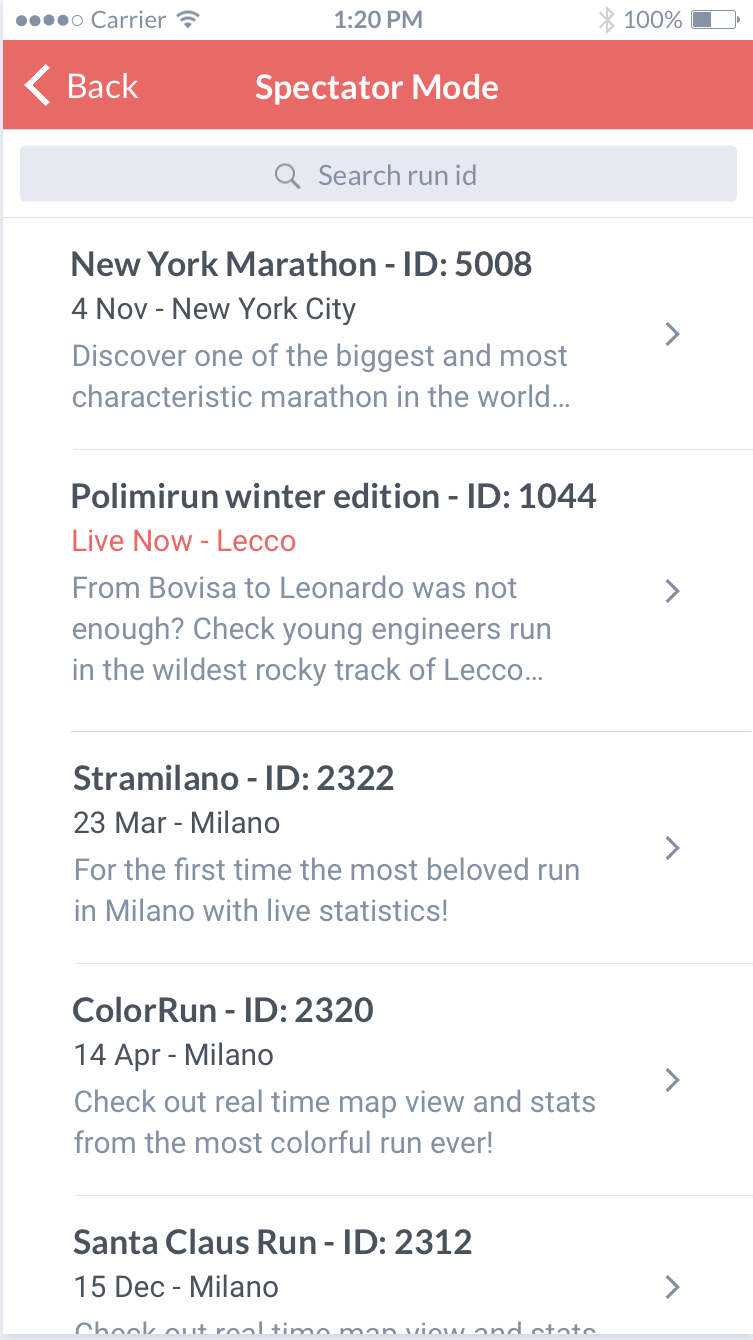
\includegraphics[width=5cm]{Mockup/mockupResearch.png}
  						\caption{Research run tab}
 					 	\label{fig:Research}
					\end{figure}

					\item[$\circ$] {\bf Selected run} \\
					After having selected a run, the {\it Spectator} will see its path and its participants’ locations live on the track. This view will be visible for the whole duration of the run.\\	
					\begin{figure}[H]
						\center
  						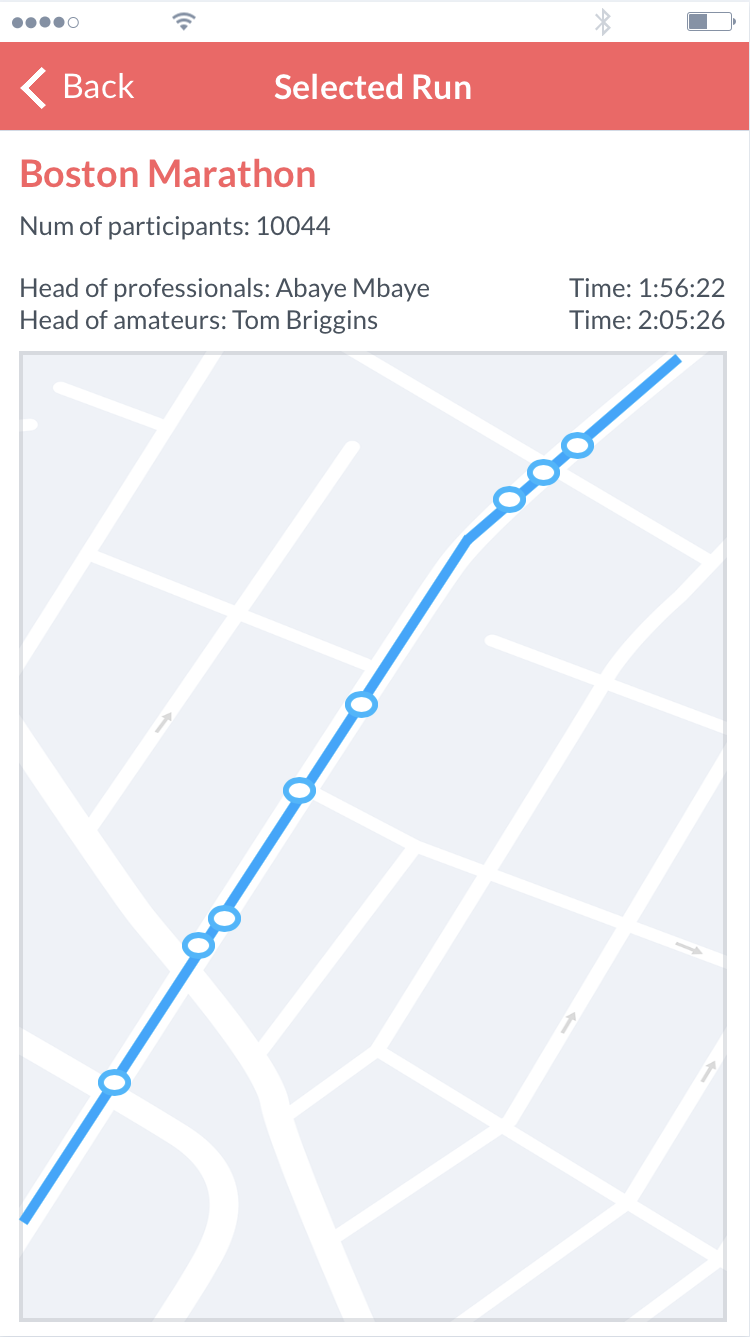
\includegraphics[width=5cm]{Mockup/mockupSelectedRun.png}
  						\caption{Selected run tab}
 					 	\label{fig:SelectedRun}
					\end{figure}
				\end{itemize}
			\end{itemize}
		\end{itemize}
						
		\subsubsection{Hardware Interfaces}
		The {\it System} doesn’t offer any Hardware Interfaces.
			
		\subsubsection{Software Interfaces}
		\begin{itemize}
			\item{\bf Operating System: } As mobile applications, the main software interfaces would be offered to the OS on which they run, in particular:
			\begin{itemize}
				\item[$\circ$] iOS
				\item[$\circ$]Android
				\item[$\circ$] Android Wear
				\item[$\circ$] WatchOS
			\end{itemize}
			\item{\bf Web Server APIs: } Functioning as endpoints offered to both {\it Data4Help} and {\it Track4Run} mobile applications to access the Web Server.
These APIs are public and can be used by {\it Third Parties} to directly access the Web Server (authentication has to be provided with each request).

		\end{itemize}
			
		\subsubsection{Communication Interfaces}
		\begin{itemize}
			\item {\bf HTTPS Protocol:} to safely communicate through the internet with the Web Server and the DBMS.

		\end{itemize}

	\subsection{Functional Requirements}
			
		\subsubsection{Use Case Diagrams}
			
		\begin{figure}[H]
  			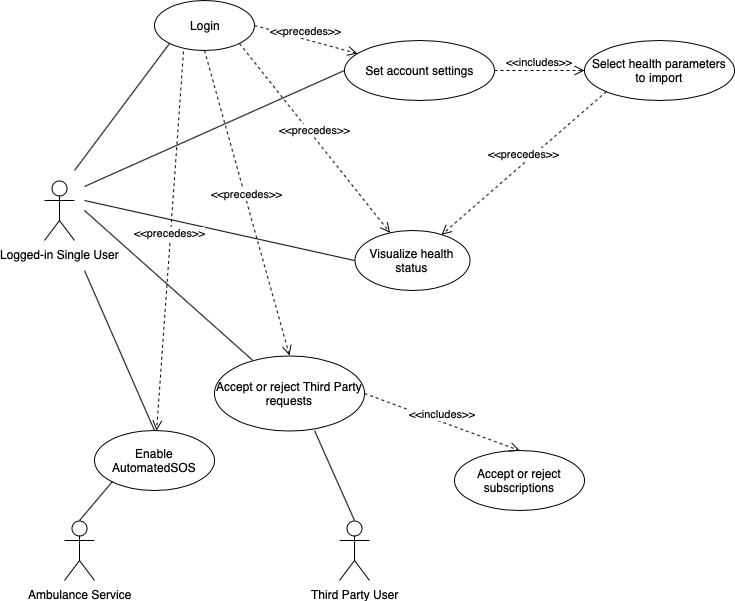
\includegraphics[width=\linewidth]{Diagrammi/SingleUserUseCase.png}
  			\caption{{\it Single User} Use Case Diagram}
 			 \label{fig:SingleUserUseCase}
		\end{figure}
			
		\begin{figure}[H]
  			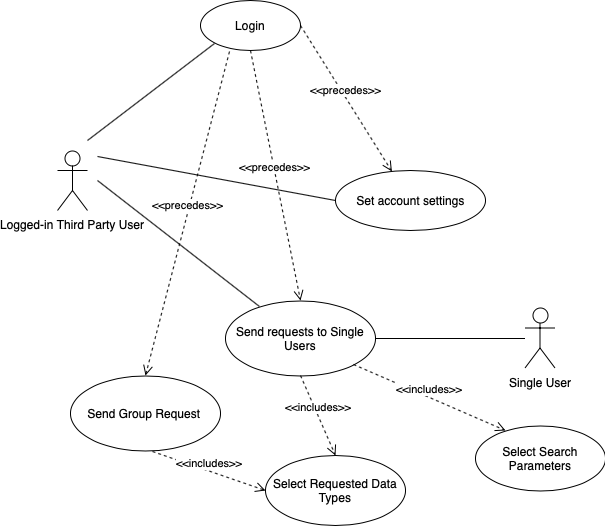
\includegraphics[width=\linewidth]{Diagrammi/ThirdPartyUseCase.png}
  			\caption{{\it Third Party} User Use Case Diagram}
 			 \label{fig:ThirdPartyUseCase}
		\end{figure}

		\subsubsection{Scenarios}
			
				\begin{itemize}
					\item {\bf Scenario 1} \linebreak
					Antonio is a 65 years old retired trader who enjoys a comfy and quiet life. 
					He jogs in the park every day to keep up his good shape. One morning he is running as usual when 					he starts feeling a bit of chest pain. John does not pay much attention and he attributes it to the 					fatigue derived from running. Suddenly he feels a strong pang at the heart level. He is having a 					severe heart attack due to excessive stress and fatigue. His heart completely stops as he falls to 					the ground. There is no-one around to call for help. Luckily Antonio has activated the Automated 					SOS feature from the {\it Data4Help} app installed on his smartphone. The app is collecting data from 					his smartwatch and as soon as it notices the sudden heart rate drop it performs a silent call to the 					emergency number providing Antonio’s position. The emergency team arrives just in time and is 					able to save Antonio with a cardiac massage.
					\item {\bf Scenario 2} \linebreak
					The San Raffaele Hospital wants to conduct a study on the average hours slept by young adults 					living in Milan compared to the those of the rest of the Lombardy’s towns. The Hospital downloads 					{\it Data4Help} and creates an account as a {\it Third Party} User. Researchers at the hospital access the 					application through this account  and decide Polto perform group requests to retrieve data 						concerning sleeping hours. 
					For the purpose of their studies, they decide to use the filtering feature provided by the application 					to select a group of users aged between 25 and 40 years old and living in the Municipality of Milan. 					In order to compare this result to the hours slept in average by all young adults in Lombardy, the 					researches perform the same group request but filter the result on the whole region. 
					Thanks to the data retrieved through {\it Data4Help}, the group discovers that young adults in Milan 					sleep an average of 1.5 hours less than their neighbors and finally publishes its report.
					\item {\bf Scenario 3} \linebreak
					Politecnico di Milano wants to organize a new Polimirun open only to students, for free. The 						organizers decide to make use of the brand new {\it Track4Run} application released by three of its 					alumnis. They sign-up with an Organizer account, create an event for the 11th November 2018 in 					Lecco, and send the identification code to all students by email. More than 5000 students want to 					take part in the event, so they sign up with a Runner account and join the run after searching it with 					the identification code received.
					Politecnico can now get rid of the sensors they placed on runner ids, as {\it Track4Run} allows the 						organizers to keep track of the path of each runner and provides in-depth statistics not only 						regarding running pace, but also heart rate for instance. 
					Last but not least, all supportive parents at home can now follow and cheer for their sons in real-					time by joining the event as {\it Spectator}s, without having the need to sign-up on the service.
					\item {\bf Scenario 4} \linebreak
					Federico was diagnosed with a severe cardiac disease for which he has been suffering for several 					years. Bob’s doctor decides to try a new a new medical cure that, alongside with a more healthy 					lifestyle, might improve Federico’s everyday life. In order to follow his patient’s progresses and 						recovery, Federico’s doctor decides to download {\it Data4Help} and suggests his patient do the same. 					While the doctor will create a {\it Third Party} account, Federico will create a {\it Single User} one. Thanks to 					this service Federico’s doctor is able to subscribe to Federico’s health data, monitor his heart rate 					on a daily basis and verify if he is increasing his active energy. All this gathered data will help him 					establish whether the cure shows any results and will allow Federico to feel safer when moving 					around. Furthermore Federico can also activate {\it AutomatedSOS}, so, whenever his disease 						threatens him the most, {\it Data4Help} will immediately discover his critical condition and call an 						ambulance.
				\end{itemize}	
			
		\subsubsection{Use Cases}
		
		%USE CASES
		
%%%%%%%%%%%%%%%%%%%%%%%%%%%%%%%%%%%%%%%%%%%%%%%%%%%%%%%%
			\begin{longtable}{| p{3 cm} | p{10 cm} |} 
			\hline
			{\bf ID} & UC1 \\
			\hline
			{\bf Description} & A {\it {\it Guest}} creates a {\it Single User} account for the application \\
			\hline
			{\bf Actors} & {\it {\it Guest}} \\
			\hline
			{\bf Preconditions} & 		
							\begin{itemize}
								\item The {\it {\it Guest}}  has downloaded the app onto his mobile device
								\item The {\it {\it Guest}}  doesn’t already have an account
							\end{itemize}
			\\
			\hline
			{\bf Flow of events} & 
							\begin{enumerate}
								\item The {\it {\it Guest}} opens the application
								\item The {\it System} asks the user to register or to login
								\item The {\it {\it Guest}} selects the register button
								\item The {\it {\it Guest}} swipes through the pages of the tutorial
								\item The {\it System}  asks which type of account the {\it {\it Guest}} wants to create
								\item The {\it {\it Guest}} selects the button corresponding to the creation of a Single 									User account
								\item The {\it System}  presents a form to fill with the user’s personal information, including FC  and credentials (email and password) 
								\item The user fills in the form
								\item The {\it System}  checks the validity of the input form
								\item The {\it Mailing {\it System}} sends the user an email to confirm its account
								\item The {\it User} receives the email and selects the URL to confirm its account
							\end{enumerate}
			
			 \\
			\hline
			{\bf Postconditions} & 
							\begin{itemize}
								\item The {\it System} has stored a new {\it Single User} account associated to the 										requesting {\it Guest}
								\item The {\it User} can access the application’s functionalities by logging in
							\end{itemize}
			\\
			\hline
			{\bf Exceptions} & 
							\begin{itemize}
								\item The {\it {\it Guest}} inputs an email that is already associated to an account. 
								\item The {\it {\it Guest}} inputs a password that doesn’t respect security constraints. 								\item The 	{\it {\it Guest}} inputs a FC that is already associated to an account. 
							\end{itemize} 
							For all the above: The {\it System} shows the user an error message and the flow of events restarts from point 7.
							\begin{itemize}
								\item The {\it {\it Guest}}  selects the login button and provides credentials that are not 									associated to any account
							\end{itemize} 
							The {\it System} shows the user an error message and the flow of events 							restarts from point 2.
							
			\\
			\hline
			\caption{Create a {\it Single User} account Use Case}
			\end{longtable}
			
%%%%%%%%%%%%%%%%%%%%%%%%%%%%%%%%%%%%%%%%%%%%%%%%%%%%%%%%	
			
			\begin{longtable}{| p{3 cm} | p{10 cm} |} 
			\hline
			{\bf ID} & UC2 \\
			\hline
			{\bf Description} & A {\it {\it Guest}} creates a {\it Third Party} account for the application \\
			\hline
			{\bf Actors} & {\it {\it Guest}} \\
			\hline
			{\bf Preconditions} & 		
							\begin{itemize}
								\item The {\it {\it Guest}}  has downloaded the app onto his mobile device
								\item The {\it {\it Guest}}  doesn’t already have an account
							\end{itemize}
			\\
			\hline
			{\bf Flow of events} & 
							\begin{enumerate}
								\item The {\it {\it Guest}} opens the application
								\item The {\it System} asks the user to register or to login
								\item The {\it {\it Guest}} selects the register button
								\item The {\it {\it Guest}} swipes through the pages of the tutorial
								\item The {\it System}  asks which type of account the {\it {\it Guest}} wants to create
								\item The {\it {\it Guest}} selects the button corresponding to the creation of a {\it Third Party} account
								\item The {\it System}  presents a form to fill with the user’s personal information, including P.IVA and credentials (email and password) 
								\item The user fills in the form
								\item The {\it System}  checks the validity of the input form
								\item The {\it Mailing {\it System}} sends the user an email to confirm its account
								\item The {\it User} receives the email and selects the URL to confirm its account
							\end{enumerate}
			
			 \\
			\hline
			{\bf Postconditions} & 
							\begin{itemize}
								\item The {\it System} has stored a new {\it Third Party} account associated to the 										requesting {\it Guest}
								\item The {\it User} can access the application’s functionalities by logging in
							\end{itemize}
			\\
			\hline
			{\bf Exceptions} & 
							\begin{itemize}
								\item The {\it {\it Guest}} inputs an email that is already associated to an account. 
								\item The {\it {\it Guest}} inputs a password that doesn’t respect security constraints. 								\item The 	{\it {\it Guest}} inputs a P.IVA that is already associated to an account. 
							\end{itemize} 
							For all the above: The {\it User Account Manager} shows the user an error message and the flow of events restarts from point 7.
							\begin{itemize}
								\item The {\it {\it Guest}}  selects the login button and provides credentials that are not 									associated to any account
							\end{itemize} 
							The {\it System} shows the user an error message and the flow of events 							restarts from point 2.
							
			\\
			\hline
			\caption{Create a {\it Third Party} Use Case}
			\end{longtable}

%%%%%%%%%%%%%%%%%%%%%%%%%%%%%%%%%%%%%%%%%%%%%%%%%%%%%%%%		
\begin{longtable}{| p{3 cm} | p{10 cm} |} 
			\hline
			{\bf ID} & UC3 \\
			\hline
			{\bf Description} & A {\it Single User} logs in\\
			\hline
			{\bf Actors} & {\it Single User} \\
			\hline
			{\bf Preconditions} & 		
							\begin{itemize}
								\item The {\it Single User}  has already created a {\it Single User} account 
							\end{itemize}
			\\
			\hline
			{\bf Flow of events} & 
							\begin{enumerate}
								\item The {\it Single User} opens the application
								\item The {\it System} asks the user to login or register
								\item The {\it Single User} selects the login button
								\item The {\it System} asks the user to input its credentials (email and password)
								\item The {\it Single User} inputs its credentials
								\item The {\it System} checks the provided credentials

							\end{enumerate}
			
			 \\
			\hline
			{\bf Postconditions} & 
							\begin{itemize}
								\item The {\it System} shows the {\it Single User}’s main interface
							\end{itemize}
			\\
			\hline
			{\bf Exceptions} & 
							\begin{itemize}
								\item The {\it Single User} inputs the wrong credentials. 
							\end{itemize}
							The {\it System} shows the user an error message and the flow of events 							restarts from point 4.
							
			\\
			\hline
			\caption{Log in a {\it Single User} Account}
			\end{longtable}

%%%%%%%%%%%%%%%%%%%%%%%%%%%%%%%%%%%%%%%%%%%%%%%%%%%%%%%%		
\begin{longtable}{| p{3 cm} | p{10 cm} |} 
			\hline
			{\bf ID} & UC4 \\
			\hline
			{\bf Description} & A {\it Third Party} logs in\\
			\hline
			{\bf Actors} & {\it {\it Third Party} User} \\
			\hline
			{\bf Preconditions} & 		
							\begin{itemize}
								\item The {\it Third Party}  has already created a {\it Third Party} account 
							\end{itemize}
			\\
			\hline
			{\bf Flow of events} & 
							\begin{enumerate}
								\item The {\it Third Party} opens the application
								\item The {\it System} asks the user to login or register
								\item The {\it Third Party} selects the login button
								\item The {\it System} asks the user to input its credentials (email and password)
								\item The {\it Third Party} inputs its credentials
								\item The {\it System} checks the provided credentials

							\end{enumerate}
			
			 \\
			\hline
			{\bf Postconditions} & 
							\begin{itemize}
								\item The {\it System} shows the {\it Third Party}’s main interface
							\end{itemize}
			\\
			\hline
			{\bf Exceptions} & 
							\begin{itemize}
								\item The {\it Third Party} inputs the wrong credentials. 
							\end{itemize}
							The {\it System} shows the user an error message and the flow of events 							restarts from point 4.
							
			\\
			\hline
			\caption{Log in a {\it Third Party} Account}
			\end{longtable}

%%%%%%%%%%%%%%%%%%%%%%%%%%%%%%%%%%%%%%%%%%%%%%%%
\begin{longtable}{| p{3 cm} | p{10 cm} |} 
			\hline
			{\bf ID} & UC5 \\
			\hline
			{\bf Description} & A {\it Single User} selects which health data to import\\
			\hline
			{\bf Actors} & {\it Logged-in {\it Single User}} \\
			\hline
			{\bf Preconditions} & 		
							\begin{itemize}
								\item The {\it Single User}  has  logged into his account 
							\end{itemize}
			\\
			\hline
			{\bf Flow of events} & 
							\begin{enumerate}
								\item The {\it Single User} selects the My Settings tab in the application
\item The {\it System} shows all the information related to the user’s account and enables modifications
\item The user selects the types of health data to import from the list displayed in the interface
							\end{enumerate}
			
			 \\
			\hline
			{\bf Postconditions} & 
							\begin{itemize}
								\item The {\it System} updates the user’s account settings 
\item The {\it System} imports data from the user’s device corresponding to the new selected types (if any)
\item The {\it System} does not import anymore the removed types (if any)

							\end{itemize}
			\\
			\hline
			{\bf Exceptions} & 
							\begin{itemize}
								\item The User has no available data related to the selected type
The {\it System} does not retrieve any data corresponding to that type

							\end{itemize}
							
			\\
			\hline
			\caption{Select types of health data to import}
			\end{longtable}

%%%%%%%%%%%%%%%%%%%%%%%%%%%%%%%%%%%%%%%%%%%%%%%%%%%%%%%%	

\begin{longtable}{| p{3 cm} | p{10 cm} |} 
			\hline
			{\bf ID} & UC6 \\
			\hline
			{\bf Description} & A {\it Single User} accepts a request from a {\it Third Party}\\
			\hline
			{\bf Actors} & {\it Logged-in {\it Single User}}, {\it Third Party} \\
			\hline
			{\bf Preconditions} & 		
							\begin{itemize}
								\item The {\it Single User}  has  logged into his account 
							\end{itemize}
			\\
			\hline
			{\bf Flow of events} & 
							\begin{enumerate}
								\item The {\it System} signals a new {\it Third Party} request with a notification on the My Follower tab icon
\item The Logged-in {\it Single User} selects the My Followers tab
\item The {\it System}  in this tab shows the user a {\it Third Party} request
\item The user reads the description of the {\it Third Party} sending the request
\item The {\it System} asks the user to accept or reject the request
\item The user accepts the request
\item The {\it System} signs the request as accepted and forwards the response to the sender
							\end{enumerate}
			
			 \\
			\hline
			{\bf Postconditions} & 
							\begin{itemize}
								\item The {\it Third Party} sending the request is added to the list of the user’s followers
\item The {\it System} retrieves the accepting {\it Single User}’s data and forwards it to the requesting {\it Third Party} 


							\end{itemize}
			\\
			\hline
			{\bf Exceptions} & 
							\begin{itemize}
								\item There is no available data related to the {\it Single User}’s account corresponding to the parameters input by the {\it Third Party}
							\end{itemize}
							The {\it System} notifies to the {\it Third Party} that there is no such data available.

							
			\\
			\hline
			\caption{Accept a {\it Third Party} Request}
			\end{longtable}

%%%%%%%%%%%%%%%%%%%%%%%%%%%%%%%%%%%%%%%%%%%%%%%%%%%%%%%%				
\begin{longtable}{| p{3 cm} | p{10 cm} |} 
			\hline
			{\bf ID} & UC7 \\
			\hline
			{\bf Description} & A {\it Single User} rejects a request from a {\it Third Party}\\
			\hline
			{\bf Actors} & {\it Logged-in {\it Single User}}, {\it Third Party} \\
			\hline
			{\bf Preconditions} & 		
							\begin{itemize}
								\item The {\it Single User}  has  logged into his account 
							\end{itemize}
			\\
			\hline
			{\bf Flow of events} & 
							\begin{enumerate}
								\item The {\it System} signals a new {\it Third Party} request with a notification on the My Follower tab icon
\item The Logged-in {\it Single User} selects the My Followers tab
\item The {\it System}  in this tab shows the user a {\it Third Party} request
\item The user reads the description of the {\it Third Party} sending the request
\item The {\it System} asks the user to accept or reject the request
\item The user rejects the request
\item The {\it System} signs the request as rejected and forwards the response to the sender
							\end{enumerate}
			
			 \\
			\hline
			{\bf Postconditions} & 
							\begin{itemize}
								\item The {\it Third Party} receives the notification from the {\it System} signaling the user’s rejection

							\end{itemize}
			\\
			\hline
			{\bf Exceptions} & 
							
			\\
			\hline
			\caption{Reject a {\it Third Party} Request}
			\end{longtable}

%%%%%%%%%%%%%%%%%%%%%%%%%%%%%%%%%%%%%%%%%%%%%%%%%%%%%%%%		

\begin{longtable}{| p{3 cm} | p{10 cm} |} 
			\hline
			{\bf ID} & UC8 \\
			\hline
			{\bf Description} & A {\it Third Party} sends a request to a {\it Single User} \\
			\hline
			{\bf Actors} & {\it Logged-in {\it Third Party} }, {\it Single User} \\
			\hline
			{\bf Preconditions} & 		
							\begin{itemize}
								\item The {\it Third Party} has logged into his account
							\end{itemize}
			\\
			\hline
			{\bf Flow of events} & 
							\begin{enumerate}
								\item The {\it Third Party} opens the Search tab in the application
\item The {\it System} asks the user to select the type of research: single request or group request
\item The {\it Third Party} selects the request to a {\it Single User}
\item They {\it System} asks the user to select the requested data types and the {\it Single User}’s ID
\item The user inputs the ID (FC or email) and the requested data types 
\item The user submits the request
\item The {\it System} checks if the input ID is valid and if any requested data type is available
\item The {\it System} forwards the request to the addressed {\it Single User}

							\end{enumerate}
			
			 \\
			\hline
			{\bf Postconditions} & 
							\begin{itemize}
								\item The {\it System} forwards the {\it Single User}’s response to the {\it Third Party} (acceptance or rejection)

							\end{itemize}
			\\
			\hline
			{\bf Exceptions} & 
							\begin{itemize}
								\item The input ID is not associated to any account
\item All requested data types of the {\it Single User} are not available.

							\end{itemize}
							For all the above: The {\it System} notifies the {\it Third Party} with an error message and the flow of events restarts from point 2.

							
			\\
			\hline
			\caption{Request Data from a {\it Single User}}
			\end{longtable}

%%%%%%%%%%%%%%%%%%%%%%%%%%%%%%%%%%%%%%%%%%%%%%%%%%%%%%%%							
\begin{longtable}{| p{3 cm} | p{10 cm} |} 
			\hline
			{\bf ID} & UC9 \\
			\hline
			{\bf Description} & A {\it Third Party} submits a Group Request \\
			\hline
			{\bf Actors} & {\it Logged-in {\it Third Party} }\\
			\hline
			{\bf Preconditions} & 		
							\begin{itemize}
								\item The {\it Third Party} has logged into his account
							\end{itemize}
			\\
			\hline
			{\bf Flow of events} & 
							\begin{enumerate}
								\item The {\it Third Party} opens the Search tab in the application
\item The {\it System} asks the user to select the type of research: single request or group request.
\item The {\it Third Party} selects group request
\item The {\it System} asks the user to select the search parameters and the selected data types
\item The user inputs the search parameters
\item The user submits the request
\item The {\it System} analyses the search parameters and checks the corresponding data in the DB
							\end{enumerate}
			
			 \\
			\hline
			{\bf Postconditions} & 
							\begin{itemize}
								\item The {\it System} sends the anonymous data matching the search parameters to the {\it Third Party}
\item The {\it Third Party} can download the researched data

							\end{itemize}
			\\
			\hline
			{\bf Exceptions} & 
							\begin{itemize}
								\item The matching data belongs to a group of not more than 1000 users.
							\end{itemize}
							The {\it System} notifies the user that the matching data corresponds to a group that is too small and therefore cannot be retrieved. The flow of events restarts from point 2.
							\begin{itemize}
								\item There is no data in the db matching the search parameters.
							\end{itemize}
							The {\it System} notifies the user that there is no available data matching the request. The flow of events restarts from point 2.
							
			\\
			\hline
			\caption{Submit a Group Request}
			\end{longtable}

%%%%%%%%%%%%%%%%%%%%%%%%%%%%%%%%%%%%%%%%%%%%%%%%%%%%%%%%		
\begin{longtable}{| p{3 cm} | p{10 cm} |} 
			\hline
			{\bf ID} & UC10 \\
			\hline
			{\bf Description} & A Logged-in {\it Single User} enables {\it AutomatedSOS}  \\
			\hline
			{\bf Actors} & {\it Logged-in {\it Single User} }\\
			\hline
			{\bf Preconditions} & 		
							\begin{itemize}
								\item The user has logged into his account
							\end{itemize}
			\\
			\hline
			{\bf Flow of events} & 
							\begin{enumerate}
								\item The Logged-in {\it Single User} selects the My Health tab in the application
\item The user selects the {\it AutomatedSOS} button to enable it
\item The {\it System} asks the user permission to access his calls
\item The user grants access to his calls

							\end{enumerate}
			
			 \\
			\hline
			{\bf Postconditions} & 
							\begin{itemize}
								\item When the user’s health parameters are critical, the {\it System} calls an ambulance to the user’s location

							\end{itemize}
			\\
			\hline
			{\bf Exceptions} & 
							\begin{itemize}
								\item The user does not grant permission to make phone calls.
							\end{itemize}
							The {\it System} displays an error and disables {\it AutomatedSOS}.							
			\\
			\hline
			\caption{Enable {\it AutomatedSOS}}
			\end{longtable}

%%%%%%%%%%%%%%%%%%%%%%%%%%%%%%%%%%%%%%%%%%%%%%%%%%%%%%%%		

\begin{longtable}{| p{3 cm} | p{10 cm} |} 
			\hline
			{\bf ID} & UC11 \\
			\hline
			{\bf Description} & A {\it Third Party} organizes a run  \\
			\hline
			{\bf Actors} & {\it Logged-in {\it Third Party} }\\
			\hline
			{\bf Preconditions} & 		
							\begin{itemize}
								\item The user has logged into his account in {\it Track4Run}
							\end{itemize}
			\\
			\hline
			{\bf Flow of events} & 
							\begin{enumerate}
								\item The user selects the New Run tab
\item The {\it System} asks the user to define the run’s details: name, starting and ending times, maximum participants
\item The user inputs the run’s details
\item The {\it System} shows the user a map on which to define the path
\item The user selects a path on the map
\item The user submits the new run
							\end{enumerate}
			
			 \\
			\hline
			{\bf Postconditions} & 
							\begin{itemize}
								\item The new run is added to the list in the Active Runs tab
\item The new run is visible to all {\it Single User}s and {\it Spectator}s

							\end{itemize}
			\\
			\hline
			{\bf Exceptions} & 
							\begin{itemize}
								\item The organizer selects a non feasible path on the map.
							\end{itemize}
							The {\it System} asks the user to select another path.						
			\\
			\hline
			\caption{Organize a run}
			\end{longtable}

%%%%%%%%%%%%%%%%%%%%%%%%%%%%%%%%%%%%%%%%%%%%%%%%%%%%%%
 \begin{longtable}{| p{3 cm} | p{10 cm} |} 
			\hline
			{\bf ID} & UC12 \\
			\hline
			{\bf Description} & A {\it Single User} joins an active run  \\
			\hline
			{\bf Actors} & {\it Logged-in {\it Single User} }\\
			\hline
			{\bf Preconditions} & 		
							\begin{itemize}
								\item The user has logged into his account on {\it Track4Run}
							\end{itemize}
			\\
			\hline
			{\bf Flow of events} & 
							\begin{enumerate}
								\item The user selects the Active Runs tab
\item The {\it System} shows the user a list of all active runs 
\item The user selects a run to join
\item On the day of the run, the {\it System} sends the user an automatic request to share his health data and position with the Organizer.
\item The User accepts the request
							\end{enumerate}			
			 \\
			\hline
			{\bf Postconditions} & 
							\begin{itemize}
								\item The User can track his position live on the run’s map in the My Run section
\item The User’s position is visible to all {\it Spectator}s 
							\end{itemize}
			\\
			\hline
			{\bf Exceptions} & 
							\begin{itemize}
								\item The user doesn’t accept the request to share his data.
							\end{itemize}
							The {\it System} shows an error message to the user saying he cannot participate to the run. The flow of events restarts from point 2.						
			\\
			\hline
			\caption{Join an active run}
			\end{longtable}

%%%%%%%%%%%%%%%%%%%%%%%%%%%%%%%%%%%%%%%%%%%%%%%%%%%%%%
 \begin{longtable}{| p{3 cm} | p{10 cm} |} 
			\hline
			{\bf ID} & UC13\\
			\hline
			{\bf Description} & A {\it Spectator} looks for a specific run to spectate  \\
			\hline
			{\bf Actors} & {\it {\it Spectator} }\\
			\hline
			{\bf Preconditions} & 		
							\begin{itemize}
								\item The {\it Spectator} has downloaded the application {\it Track4Run}
							\end{itemize}
			\\
			\hline
			{\bf Flow of events} & 
							\begin{enumerate}
								\item The User opens {\it Track4Run}
\item The {\it System} asks the user to login, register or access the service as a {\it Spectator}
\item The User selects to access as a {\it Spectator}
\item The {\it System} asks the User to find a run by its identifier or to search in the list of active runs
\item The User inserts the run’s identifier
\item The User submits its research
							\end{enumerate}			
			 \\
			\hline
			{\bf Postconditions} & 
							\begin{itemize}
								\item The user can spectate the run and see its participants’ live positions

							\end{itemize}
			\\
			\hline
			{\bf Exceptions} & 
							\begin{itemize}
								\item The identifier input by the user is not associated to any existing run
							\end{itemize}
							The {\it System} shows an error message to the user. The flow of events restarts from point 4.					
			\\
			\hline
			\caption{Spectate a run}
			\end{longtable}

%%%%%%%%%%%%%%%%%%%%%%%%%%%%%%%%%%%%%%%%%%%%%%%%%%%%%%%%																								
		
			\subsubsection{Sequence Diagrams}
			The first Sequence Diagrams models the creation of a new account on {\it Data4Help}. The two actors involved are a guest user and the {\it System}. We assume the guest to be a generic user as the same procedure is applicable to both users wanting to create a Third Party account and a {\it Single User} account. Furthermore, the same sequence of events occurs when registering through {\it Track4Run}.
			\begin{figure}[H]
			\center
  			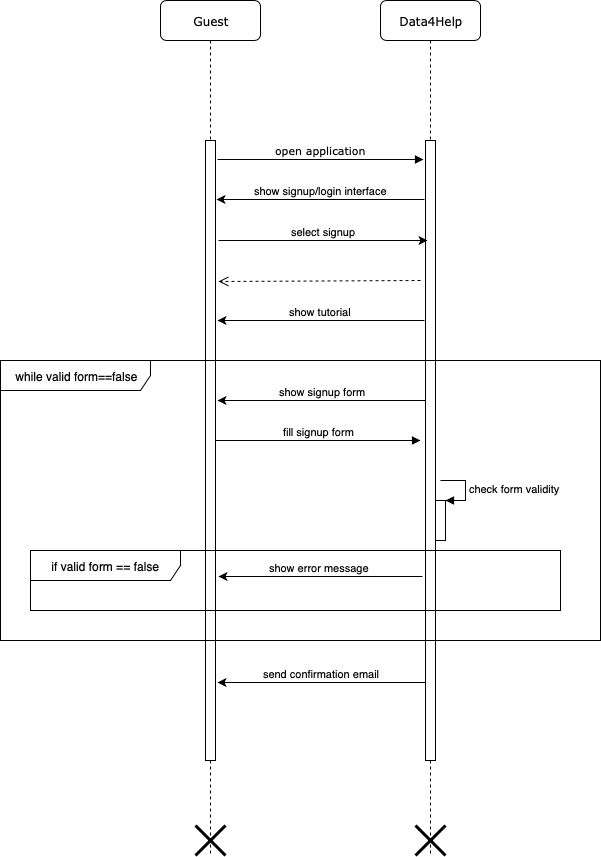
\includegraphics[width=\textwidth]{Diagrammi/sd1.png}
			\caption{Create an account}
			\label{fig:sd1}
		\end{figure} 		
The following diagram describes the sequence of events to be performed in order for a user to log into his account. As in the previous diagram, we shall consider a generic user since this procedure is the same for logging into a {\it Third Party} account or a {\it Single User} account. 
\begin{figure}[H]
			\center
  			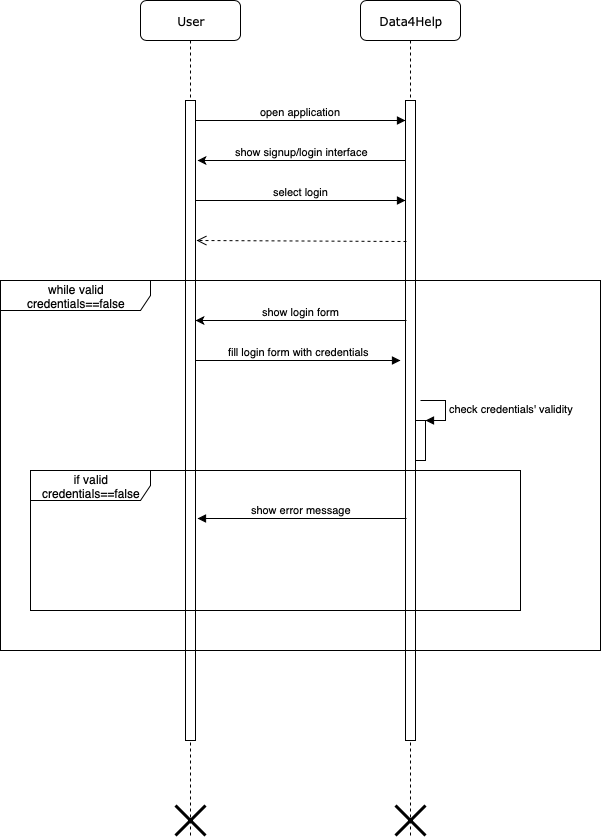
\includegraphics[width=\textwidth]{Diagrammi/sd2.png}
			\caption{Log in}
			\label{fig:sd2}
\end{figure}
The following diagram describes the procedure that occurs whenever a {\it Third Party} wants to send a request to a {\it Single User}. The actor involved in this scenario are a {\it Third Party}, a {\it Single User} and the {\it System}.
\begin{figure}[H]
			\center
  			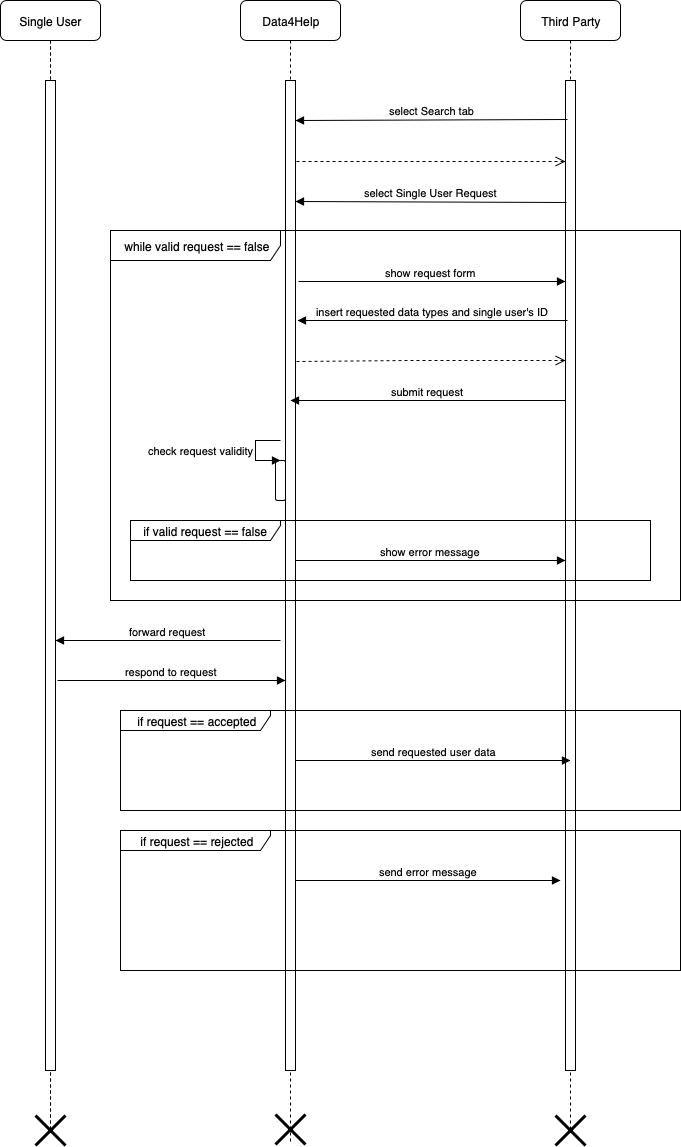
\includegraphics[width=\textwidth]{Diagrammi/sd3.png}
			\caption{Send a {\it Single Request}}
			\label{fig:sd3}
\end{figure}
In this diagram we describe the sequence of procedures that are activated when a {\it Third Party} sends a group request to the {\it System}. In this case no single users are involved, thus resulting in a two-actor scenario: a {\it Third Party} and the {\it System}.
\begin{figure}[H]
			\center
  			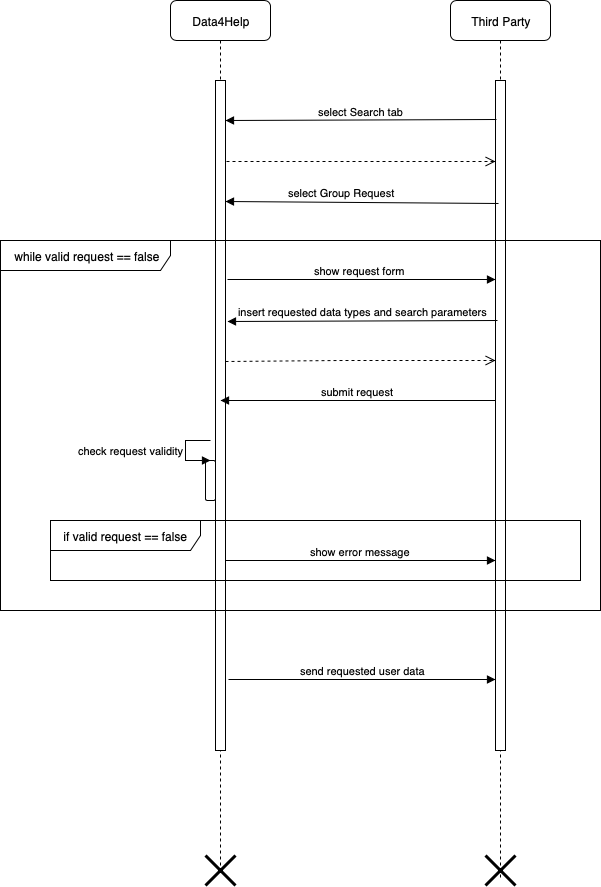
\includegraphics[width=\textwidth]{Diagrammi/sd4.png}
			\caption{Send a {\it Group Request}}
			\label{fig:sd4}
\end{figure}
The following diagram describes the sequence of events to be performed in order for a single user to enable {\it AutomatedSOS}. While modeling this feature activation, we also describe how it works when critical parameters are observed by the {\it System}. Therefore in this case our actors are a {\it Logged-in Single User}, the {\it System} and the {\it Ambulance Service}.
\begin{figure}[H]
			\center
  			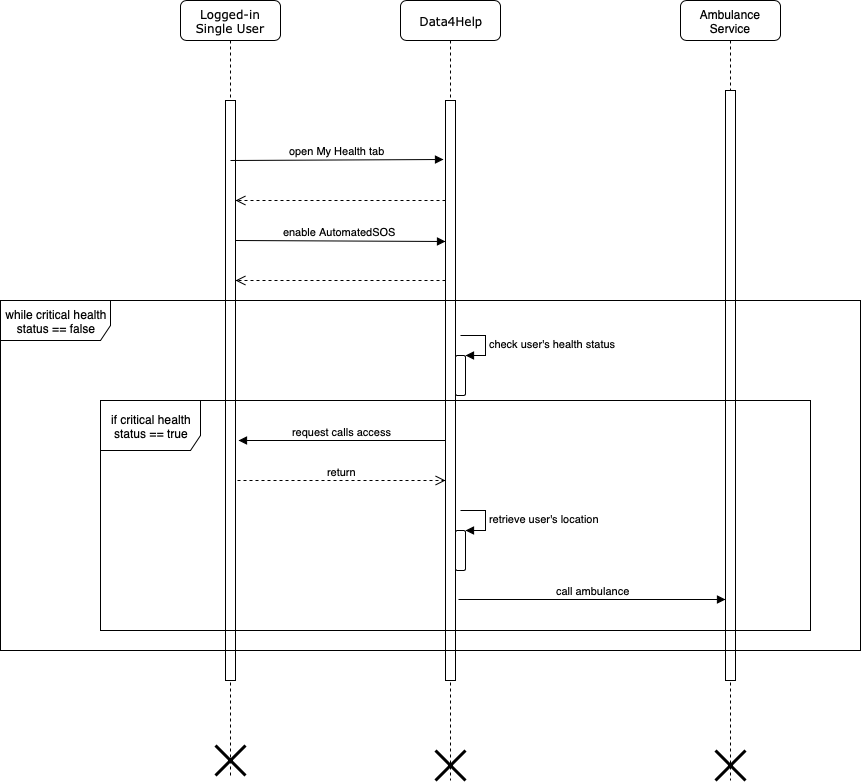
\includegraphics[width=\textwidth]{Diagrammi/sd5.png}
			\caption{Enable {\it AutomatedSOS}}
			\label{fig:sd5}
\end{figure}
The next diagram describes the sequence of events that occur whenever a {\it Third Party} organizes a new run in {\it Track4Run}. The {\it Third Party} and the {\it System} are the only actors involved.
\begin{figure}[H]
			\center
  			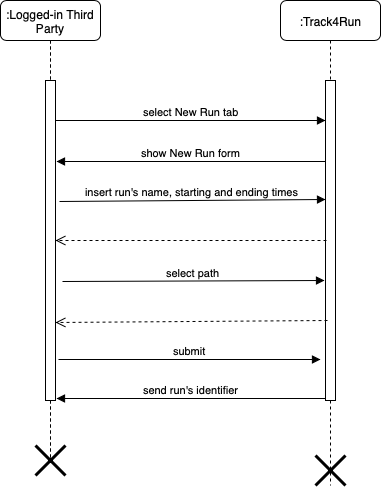
\includegraphics[width=\textwidth]{Diagrammi/sd6.png}
			\caption{Organize a run}
			\label{fig:sd6}
\end{figure}
The following digram represents the sequence of events that occur when a {\it Single User} decides to join an existing run in {\it Track4Run}. The actors involved in the scenario are only the {\it Single User} and the {\it System}.
\begin{figure}[H]
			\center
  			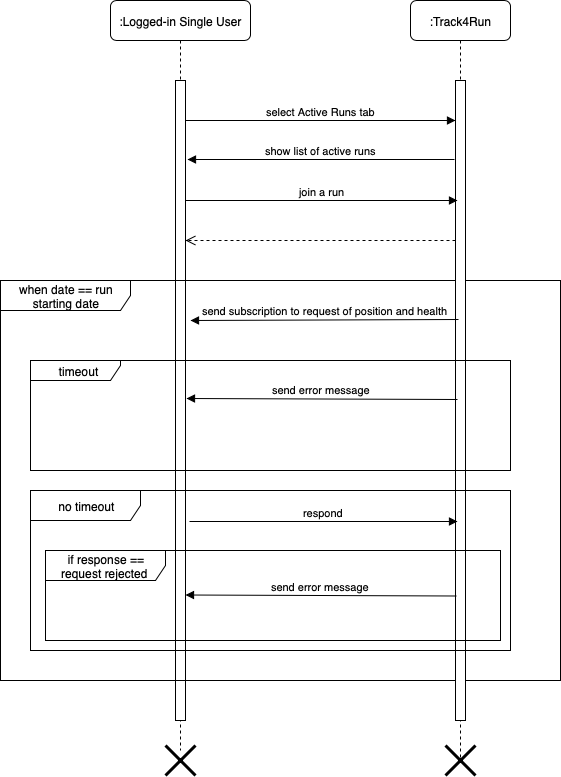
\includegraphics[width=\textwidth]{Diagrammi/sd7.png}
			\caption{Join a run}
			\label{fig:sd7}
\end{figure}
The final diagram shows the sequence of events that occur when a {\it Spectator} uses {\it Track4Run} to spectate an existing run. The {\it Spectator} and the {\it System} are the only actors involved in the scenario.
\begin{figure}[H]
			\center
  			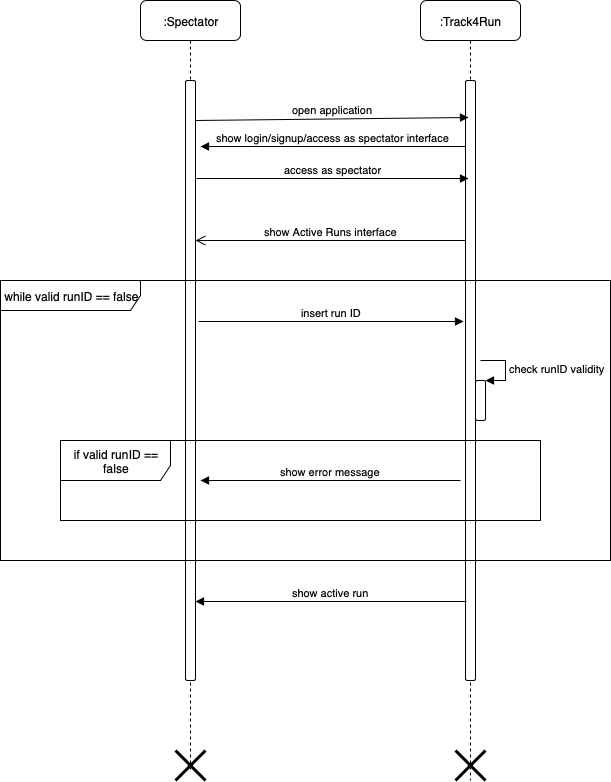
\includegraphics[width=\textwidth]{Diagrammi/sd8.png}
			\caption{Spectate a run a}
			\label{fig:sd8}
\end{figure}

									
			\subsubsection{Goal mapping on requirements}
			
			\begin{itemize} %GOALS

   				 \item {\bf [G1]} Users can be identified either as {\it {\it Single User}s} or as {\it Third Parties}.	
				 
				 	\begin{itemize} %mapping
						\item {\bf[R1]} The S2B allows users to create either a {\it Single User} or a {\it Third Party} account. 
\item {\bf[R2]}  A {\it Single User} account can be created if and only if the user provides his Fiscal Code. 
\item {\bf[R3]}  A {\it Third Party} account can be created if and only if a valid P.IVA is provided. 
\item {\bf[R4]}  All users can create an account if and only if they provide a unique email and a password. 
\item {\bf[R5]}  To access the service users must log in with their account credentials. 
\item {\bf[D1]}  Each user will create only one account.
\item {\bf[D2]}  The FC and email provided during registration are valid and belong to the person who’s creating the account.
\item {\bf[D3]}  The P.IVA and email of a {\it Third Party} are valid and specific to that company.
					\end{itemize}
   				 \item {\bf [G2]}  {\it {\it Single User}s} can have their data monitored by {\it Third Parties} for medical purposes.
				 
					 \begin{itemize} %mapping
					 	\item {\bf [R6]} The S2B allows users to manually insert Health data.
						\item {\bf [R7]} The S2B automatically imports new data whenever the application is opened.
\item {\bf [R8]}  When the application is open, the S2B continuously imports data in background.
\item {\bf [R9]}  The S2B binds collected data only to the user’s account that imported it. 
\item {\bf [R10]} {\it Third Parties} can submit a request to access data of a {\it Single User}. 
\item {\bf [R11]}  Requests concerning {\it Single User}s must specify either the email or the FC of the desired user. 
\item {\bf [R12]} Requests concerning {\it Single User}s are forwarded only to the specified user. 
\item {\bf [R13]}  A user can accept or refuse requests forwarded to him. 
\item {\bf [R14]}  {\it Third Parties} can access user’s data if and only if their request is accepted by said user. 
\item {\bf [D4]}  Data provided to the {\it System} is related to the person whose account was used to provide it.
\item {\bf [D5]}  All health data directly provided by the user represents his real health status.
\item {\bf [D7]}  Health data has a relative error lower than 5%.
\item {\bf [D8]}  Permission to access health and GPS data is always granted to the S2B.
\item {\bf [D9]} {\it Third Parties} collect data only for medical purposes.
					\end{itemize}

   				 \item {\bf [G3]} {\it {\it Single User}s} can visualize a summary of their health status
				 
					 \begin{itemize} %mapping
					 	\item {\bf [R6]} The S2B allows users to manually insert Health data.
\item {\bf [R7]}The S2B automatically imports new data whenever the application is opened.
\item {\bf [R8]}When the application is open, the S2B continuously import data in background.
\item {\bf [R9]} The S2B binds collected data only to the user’s account that imported it. 
\item {\bf [R15]} The S2B allows {\it Single User}s to visualize their historical data using Time Series. 
\item {\bf [R16]} The S2B allows {\it Single User}s to visualize their historical data using aggregated statistical operators. 
\item {\bf [R17]}The S2B allows {\it Single User}s to visualize their historical data over multiple timespans.
\item {\bf [D4]} Data provided to the {\it System} is related to the person whose account was used to provide it.
\item {\bf [D5]} All health data directly provided by the user represents his real health status.
\item {\bf [D7]} Health data has a relative error lower than 5\%.
\item {\bf [D8]}Permission to access health and GPS data is always granted to the S2B. 
\item {\bf [D14]} Users’ smartphones always have internet access when the S2B needs it.

					\end{itemize}
   				 \item {\bf [G4]} {\it Third Parties} can access data of those {\it Single User}s who granted their permission.
				 \begin{itemize} %mapping
				 	\item {\bf [R10]} {\it Third Parties} can submit a request to access data of a {\it Single User}. 
\item {\bf [R11]} Single Requests must specify either the email or the FC of the desired user.
\item {\bf [R12]} Single Requests are forwarded only to the specified user. 
\item {\bf [R13]}A user can accept or refuse requests forwarded to him. 
\item {\bf [R14]} {\it Third Parties} can access user’s data if and only if their request is accepted by said user. 
\item {\bf [R18]} Single requests must specify the requested data types. 
\item {\bf [R19]} A request to a {\it Single User} must specify whether or not the {\it Third Party} is subscribing to that request of data.
\item {\bf [R20]} Subscriptions to requests must specify a duration.
\item {\bf [R21]} Subscriptions to requests can be ended by both the {\it Third Party} and the {\it Single User} at any time.
\item {\bf [R22]} If none of the requested data types of the {\it Single User} is available, the {\it Third Party} receives an error message.
\item {\bf [R23]} {\it Third Parties} can access only the requested data types that are available.
\item {\bf [R24]} {\it Third Parties} can download all data obtained through requests on their devices or have it sent by email.
\item {\bf [D8]} Permission to access health and GPS data is always granted to the S2B.
\item {\bf [D9]}{\it Third Parties} collect data only for medical purposes.
\item {\bf [D10]} Data is stored on persistent memory. 
\item {\bf [D11]}The storage {\it System} is fully replicated and fault-tolerant, so that a copy of a specific piece of data is always available
					 
					\end{itemize}

   				 \item {\bf [G5]} {\it Third Parties} can access data of anonymous groups of users.
				  \begin{itemize} %mapping
					 	\item {\bf [R25]} {\it Third Parties} can submit a group request to access data of groups of users. 
\item {\bf [R26]}  Group requests must include at least one search parameter. 
\item {\bf [R27]}  Group requests must specify the requested data types. 
\item {\bf [R28]}  Group request results are provided if and only if the number of users matching the search parameters is higher than 1000. 
\item {\bf [R29]} Group request results include only the data retrieved by the {\it System} matching the search parameters. 
\item {\bf [R30]} Sensitive data is excluded from group request results. 
\item {\bf [R31]} All group requests must specify whether the {\it Third Party} is subscribing to that request of data. 
\item {\bf [R20]} Subscriptions to requests must specify a duration.
\item {\bf [R32]}  Subscriptions to requests can be ended by the {\it Third Party} at any time.
\item {\bf [R24]}  {\it Third Parties} can download all data obtained through requests on their devices or have it sent by email.
\item {\bf [D8]}  Permission to access health and GPS data is always granted to the S2B.
\item {\bf [D9]} {\it Third Parties} collect data only for medical purposes.
\item {\bf [D10]} Data is stored on persistent memory. 
\item {\bf [D11]}  The storage {\it System} is fully replicated and fault-tolerant, so that a copy of a specific piece of data is always available.
									
					\end{itemize}

   				 \item {\bf [G6]} Whenever a user’s health status becomes critical, an ambulance is sent to his location.
				 
					 \begin{itemize} %mapping
					 	\item {\bf [R33]} Only private users can choose whether or not to enable {\it AutomatedSOS}. 
\item {\bf [R34]} {\it AutomatedSOS} can be enabled only if the user grants permission to make emergency phone calls. 
\item {\bf [R35]} If {\it AutomatedSOS} is enabled and the {\it System} detects that a user’s heart rate is below or above the critical threshold for his age, an ambulance is called. 
\item {\bf [D4]} Data provided to the {\it System} is related to the person whose account was used to provide it.
\item {\bf [D5]} All health data directly provided by the user represents his real health status.
\item {\bf [D6]}Position data has an accuracy of 10 meters around the actual position.
\item {\bf [D7]} Health data has a relative error lower than 5%.
\item {\bf [D8]}Permission to access health and GPS data is always granted to the S2B.
\item {\bf [D12]} Permission to make calls is always granted to the S2B.
\item {\bf [D13]} Users’ smartphones always have signal when needed by {\it AutomatedSOS}.
					\end{itemize}
					
					 \item {\bf [G7]}  Organizers can create and manage runs.
				 
					 \begin{itemize} %mapping
					 	\item {\bf [R36]} The S2B allows organisers to create a {\it Third Party} account using {\it Data4Help}.
\item {\bf [R37]} Only {\it Third Parties} can create a run.
\item {\bf [R38]} When creating a run, the organiser must specify its the path, duration and maximum participants.
\item {\bf [R39]} On the day of a run the S2B sends a Single Request to every user who has registered to that run.
\item {\bf [R40]}The request is sent on behalf of the organiser using its email and P.IVA.
\item {\bf [R41]} The request sent is with a subscription that lasts until the end of the run.
\item {\bf [R42]}The request sent by the S2B has as requested data types the position and all available health parameters of the user.
\item {\bf [R43]}The S2B provides a list of all existing runs visible to everyone using {\it Track4Run}.
\item {\bf [D15]} The path specified when creating a run is feasible. 

					\end{itemize}
					
					\item {\bf [G8]}  Runners can enroll in an existing run.
				 
					 \begin{itemize} %mapping
					 	\item {\bf [R44]} The S2B allows runners to create a {\it Single User} account using {\it Data4Help}.
\item {\bf [R45]} Only users with a {\it Single User} account can join an existing run.
\item {\bf [R43]} The S2B provides a list of all existing runs visible to everyone using {\it Track4Run}.
\item {\bf [R46]}A user can only join a run in the list provided by the S2B.
\item {\bf [R47]} A user can’t check-in for a run if he doesn’t accept the request received by the organiser of such run.
\item {\bf [R48]} A user can’t accept the request if he doesn’t have at least his position available as requestable data type.
\item {\bf [R49]} If a user fails to check-in in the run, the S2B removes him from it.
\item {\bf [D8]} Permission to access health and GPS data is always granted to the S2B.

					\end{itemize}
					
					\item {\bf [G9]}  Organizers can create and manage runs.
				 
					 \begin{itemize} %mapping
					 	\item {\bf [R50]} An existing run can be spectated without logging in the {\it System}.
\item {\bf [R43]} The S2B provides a list of all existing runs visible to everyone using {\it Track4Run}.
\item {\bf [R51]} An existing run can be spectated by selecting it in the list of existing runs.
\item {\bf [R52]} {\it Spectator}s can see the live position of all runners participating in the run they are spectating.
\item {\bf [D6]}Position data has an accuracy of 10 meters around the actual position.
\item {\bf [D14]} Users’ smartphones always have internet access when the S2B needs it.
					\end{itemize}
				 
			\end{itemize}
			
		
		\subsection{Performance Requirements}
		In this section we will specify some static and dynamic numerical requirements attributed to the {\it System} or to the 	interaction between the human user and the application that highlight the performance reachable by the machine. \\
	Regarding static numerical requirements the {\it System} can support up to 1 million registered users. This limitation is not 	posed by the front-end of the {\it System}, but rather by the back-end part, specifically the DB.\\
	Data exchanged is only textual and for each user the {\it System} provides enough space to store up to 10Mb of data. If the 	stored information exceeds this limitation then the oldest pieces will be overwritten.\\
	All the requests that need  a direct confirmation from {\it Single User}s will have a response time of at most 3 days. If at the 	end of this period the request is still pending it will be automatically denied.\\
	Requests about groups of users shall be processed in less than 5 seconds.\\
	Requests about subscribed {\it Single User}s shall be processed in less than 1 second.\\
	The {\it AutomatedSOS} feature does not need to communicate with the back-end; also its role is much more critical given 	the function it provides and therefore the response time of this subSystem will be of 0.5 seconds starting from the 		moment it observes critical health parameters for the first time.\\
	Finally, speaking of dynamical numerical requirements the {\it System} as a whole should not be subject to peak workload 	conditions; data is retrieved from the end user at a fixed rate and the data requests from {\it Third Parties} only represent a 	minimum percentage of the data exchanged and processed between the {\it System}’s front-end and back-end.\\
	
		\subsection{Design Constraints}
		
			\subsubsection{Standards compliance}
			Our {\it System} will be compliant with standard D0-178C. This means that all software testing will be driven from 			requirements, thus enabling to link each single requirement the test case used to verify if it has been met.\\
			In our case we consider the S2B as a level D risk level {\it System} in regard to D0-178C. Therefore we can trace 			{\it System} and high level requirements to the test cases, test procedures and test results.\\
			The data format used to track all the variables is the following:
			\begin{itemize}
				\item BPM for heart rate, which is the most common unit of measurement that can be found in the 					medical field.
				\item Standard {\it SI} measurement units for height and  weight, namely meters and kilograms.
				\item Standard longitude and latitude measures for the position.
			\end{itemize}
		
			\subsubsection{Hardware limitations}
			To be able to perform as intended, the application should run in a hardware environment that guarantees the 			following specifications:
			\begin{itemize}
				\item 100Mb of mass memory 
				\item 20Mb/s wireless internet connection
				\item 2Gb of Ram 
			\end{itemize}
						
			
		\subsection{Software System Attributes}
			\subsubsection{Availability}
			Given the integration of {\it AutomatedSOS} in {\it Data4Help} and assuming that at least one user has the service 			activated, the Availability should be high. This has to hold for all users, since it is not possible to adapt it to 			each of them. Therefore the target value is 99\%. \\
			{\it Track4Run} ideally requires a lower availability, but since part of the back-end is shared with {\it Data4Help}, the 			target value should stay the same.\\
			\subsubsection{Reliability}
			The Reliability of {\it Data4Help}, like the Availability, should be high enough to guarantee the nonfunctional 				requirements of {\it AutomatedSOS}. To prevent downtime, one of the main goals of architecture design must be 			ensuring graceful degradation of the {\it System}.\\
			This holds for {\it Track4Run} as well, since downtime during a run would be a severe service disruption.\\
			\subsubsection{Security}
			Security is a key feature in a {\it System} that holds sensitive data. Thus, the S2B must:
			\begin{enumerate}
				\item As previously stated, use HTTPS to safely communicate with the Server and DBMS.
				\item Hash the passwords so that they are not stored in clear in the DB.
				\item Encrypt sensitive data before storing it to reduce the effects of data leaks.
				\item Prevent {\it Third Parties} from accessing sensitive data with group requests.
			\end{enumerate}
			\subsubsection{Maintainability}
			Good software engineering practices must be followed to reduce coupling, avoid code duplication and ensure 			that modules are self-sustainable. These three practices will guarantee Maintainability.\\
			\subsubsection{Portability}
			The implementation of the S2B as a mobile application ensures itself portability with regards to the user, since 			a porting from Android to iOS, and {\it vice versa}, would be quite natural. For what concerns the back-end 			part, it should be OS independent and easily reused with other hosts. \\
	
	\pagebreak	
		
%Formal analysis with Alloy
	\section{Formal analysis with Alloy}
		
		\subsection{Overview}
		We decided to use two alloy models that focus on two different aspects of the S2B.\\
		\\
		The first one is a very simple static model that formalizes {\bf [G1]} and the requirements used to entail it. The 			purpose of this first model is to create a possible view of the {\it System} in its lifecycle, when some accounts have 			already been created, and to check that requirements regarding uniqueness are satisfied. \\
		This model doesn’t describe all the components and actors, it just serves as a first-look on the main entities used in 		the second model.\\
		\\
		The second one is a more in-depth dynamic model that formalizes the main aspects of {\bf [G4]} and {\bf [G5]}. This 		model is derived from the first one by relaxing some constraints on uniqueness in order to represent dynamicity 		when creating both single and group requests.\\
		This model is intended to be used only through its predicates, and not with a generic show to create a possible 		world.\\
		\\
		In order to make generated worlds easier to understand, all relations that were not relevant for that specific world 		have been removed from the graphs.\\
		
		\subsection{Static Model}
		\begin{figure}[H]
			\center
  			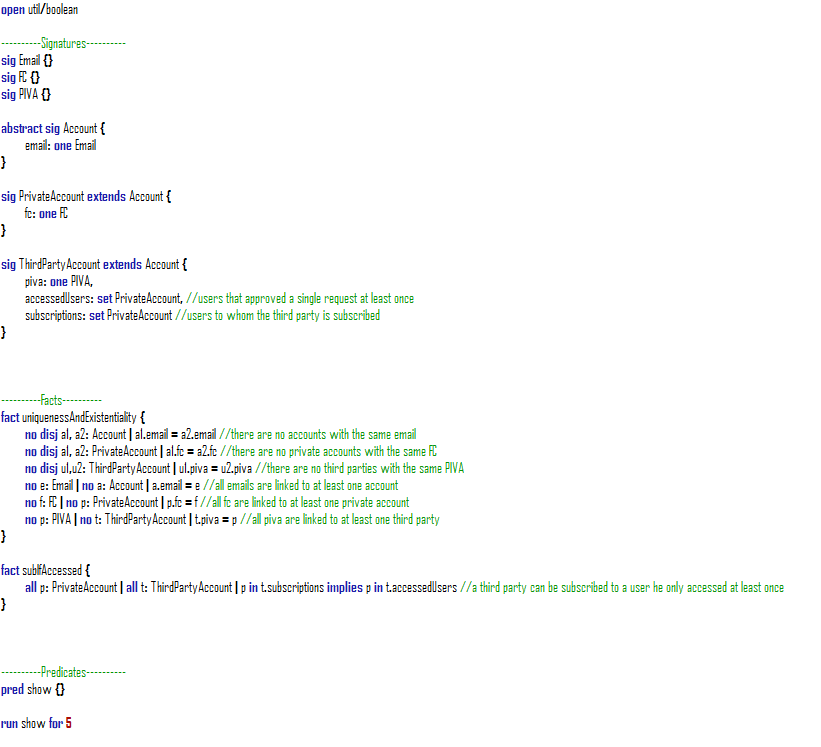
\includegraphics[width=\textwidth]{Alloy/staticAlloy.png}
			\label{fig:staticAlloy}
		\end{figure}

		\begin{figure}[H]
			\center
  			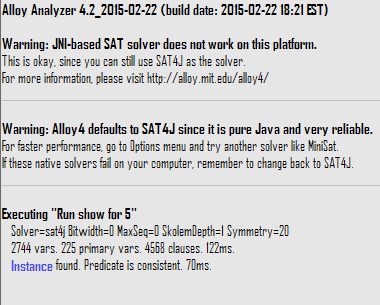
\includegraphics[width=\textwidth]{Alloy/staticCheck.png}
 			\label{fig:staticCheckl}
		\end{figure}
		
		\begin{figure}[H]
			\center
  			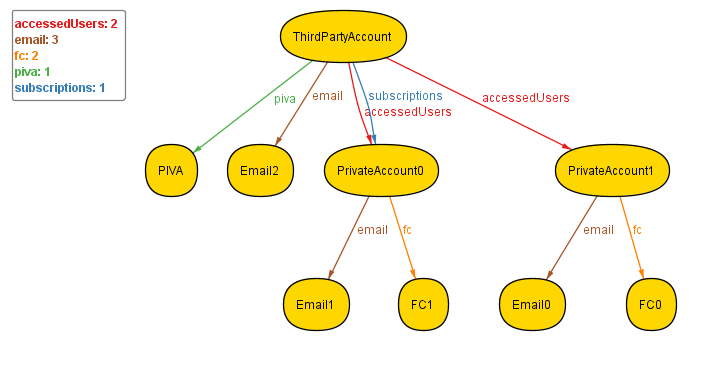
\includegraphics[width=\textwidth]{Alloy/staticModel.png}
  			\caption{Alloy Static Model}
 			\label{fig:staticModel}
		\end{figure}
	
		\subsection{Dynamic Model}
		As stated in the Overview, uniqueness constraints have been dropped in order to represent an entity before and 		after an event has occurred, in particular we’re considering as events the submission, approval and refusal of a 		request.\\
		\\
		All requests must specify the email of the sender, and have a status (Pending, Declined, Approved) and a boolean 		indicating whether the sender is subscribing to the Private Account or to the type of group request in general. The 		request data type is omitted since it’s not relevant in this model.\\
		{\it SingleRequests} must also include the P.IVA of the sender, and only one between the FC and email of the 			receiver.\\
		{\it GroupRequests} must include the search parameter used to target a group of individuals. To make things easier, 		the only possible type of condition we modeled is, for example, “All the users who have a height of 160cm”. The 		request is approved by the {\it System} only if at least 3 existing private users have a height of exactly 160cm, in this 		case we’re not modeling user evolution in time, so we assume that the number of user is fixed.\\
		\\
		The health parameters taken into consideration are Age, Heart Rate and Height, all represented as integers with a 		positive value.\\
		\\
		As an addition to the first model, all Private Accounts must have an Age, Height and the last recorded value for the 		Heart Rate. Also, each account keeps track of the pending, approved and declined single requests, which are 			disjoint one another.\\	
		\begin{figure}[H]
			\center
  			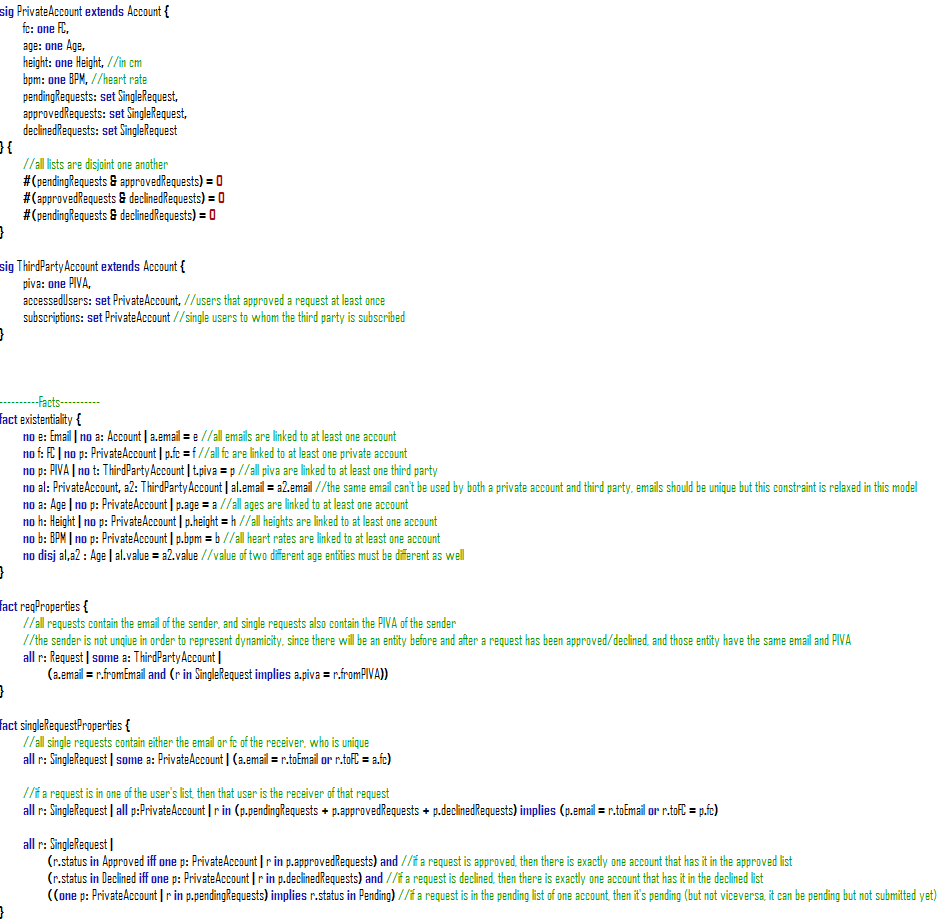
\includegraphics[width=\textwidth]{Alloy/Dynamic1.png}
			\label{fig:dyn1}
		\end{figure}

		\begin{figure}[H]
			\center
  			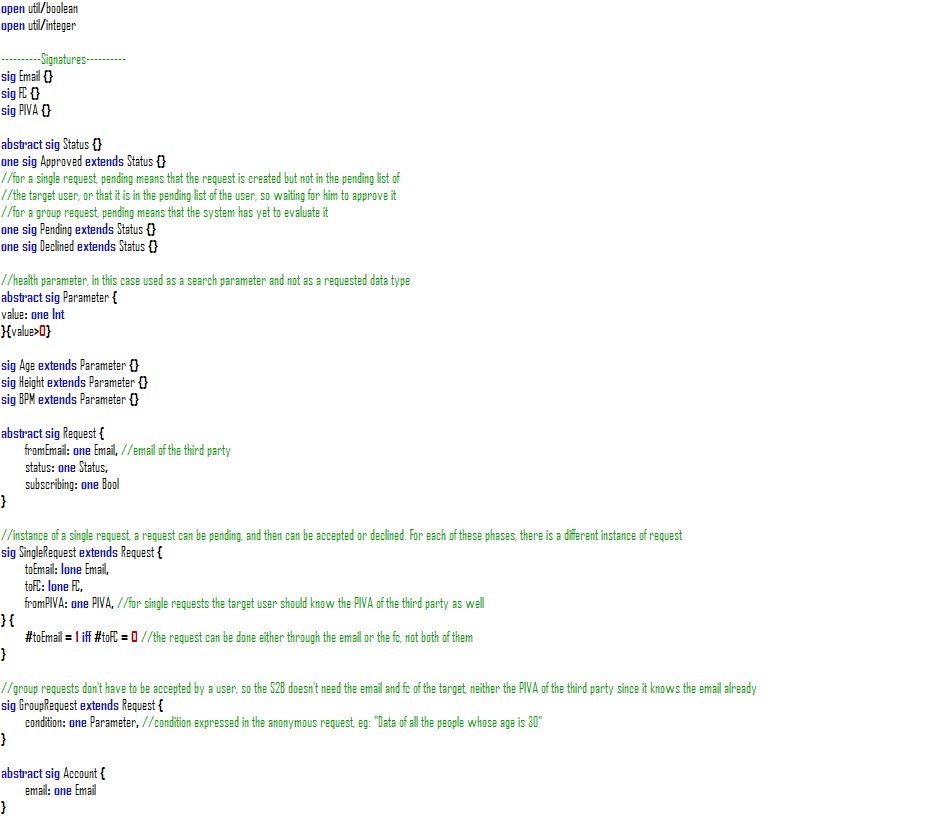
\includegraphics[width=\textwidth]{Alloy/Dynamic2.png}
			\label{fig:dyn2}
		\end{figure}

		\begin{figure}[H]
			\center
  			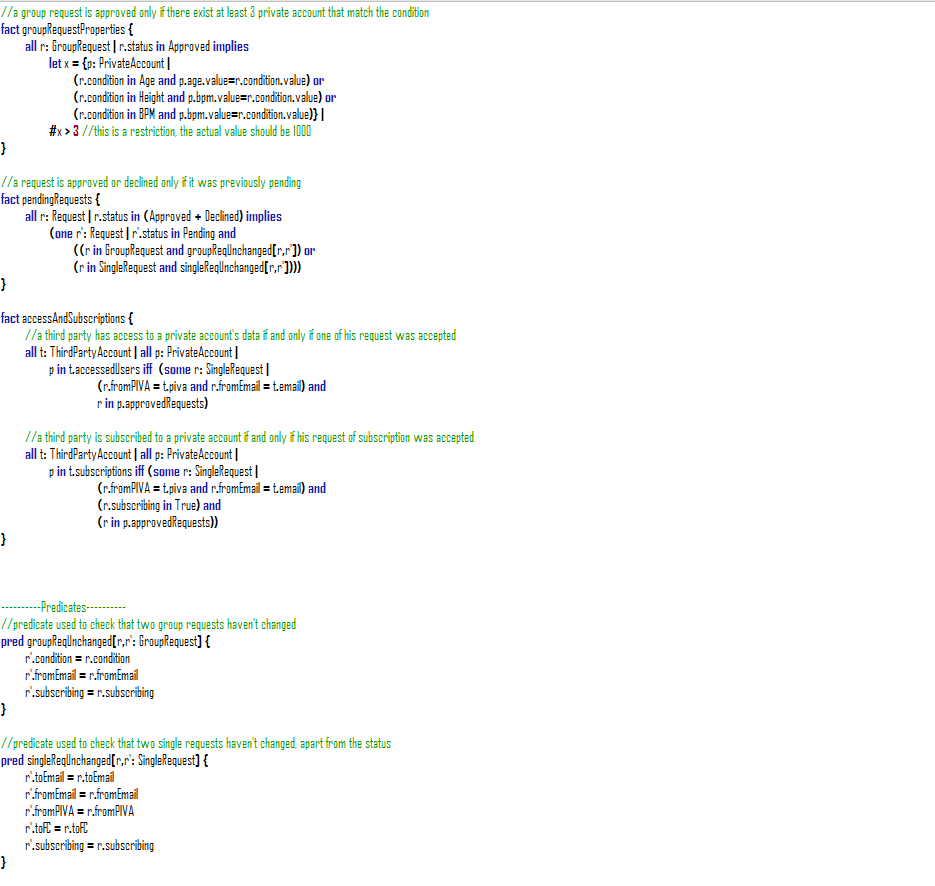
\includegraphics[width=\textwidth]{Alloy/Dynamic3.png}
			\label{fig:dyn3}
		\end{figure}

		\begin{figure}[H]
			\center
  			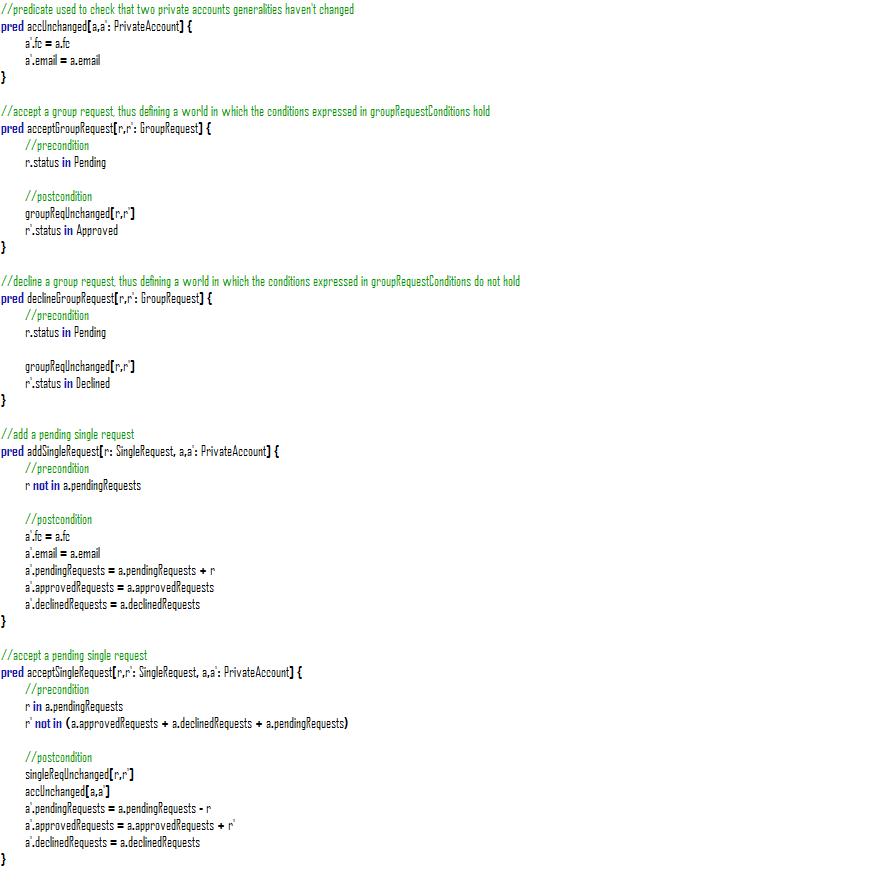
\includegraphics[width=\textwidth]{Alloy/Dynamic4.png}
			\label{fig:dyn4}
		\end{figure}

		\begin{figure}[H]
			\center
  			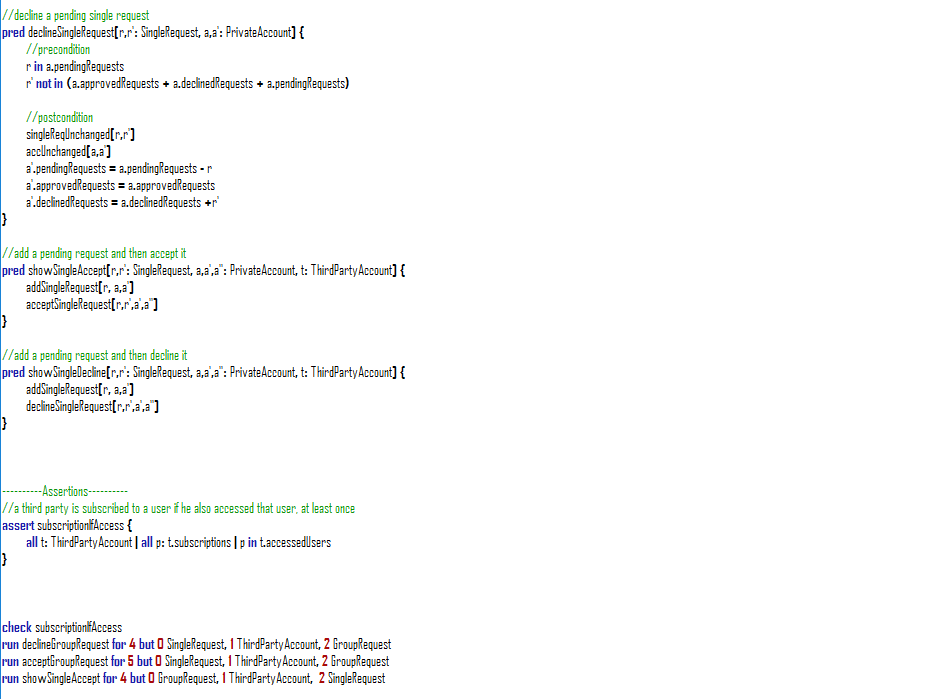
\includegraphics[width=\textwidth]{Alloy/Dynamic5.png}
			\label{fig:dyn5}
		\end{figure}

		\begin{figure}[H]
			\center
  			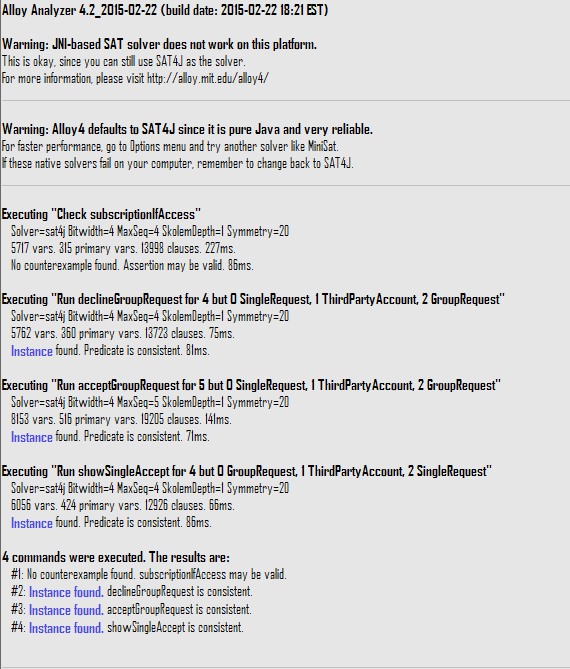
\includegraphics[width=\textwidth]{Alloy/Dynamic6.png}
			\label{fig:dyn6}
		\end{figure}

		\begin{figure}[H]
			\center
  			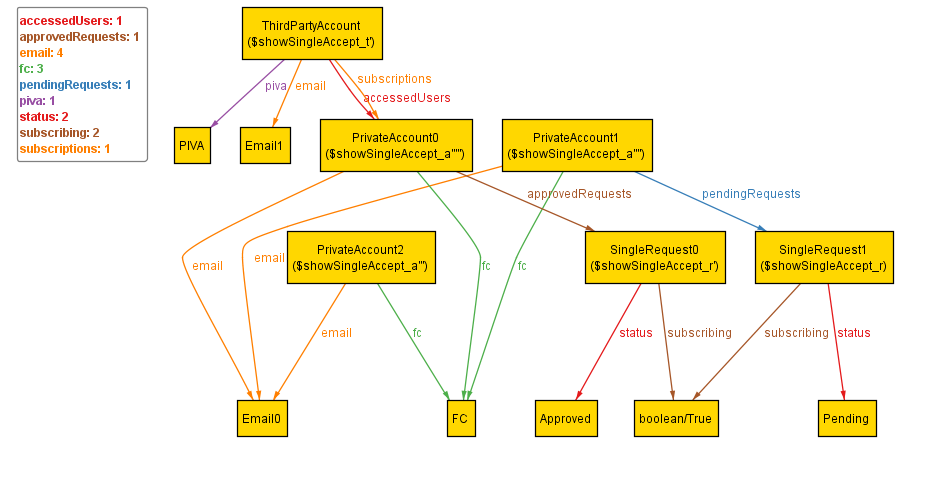
\includegraphics[width=\textwidth]{Alloy/singleRequest.png}
			\caption{Approved Single Request}
			\label{fig:sing}
		\end{figure}

		\begin{figure}[H]
			\center
  			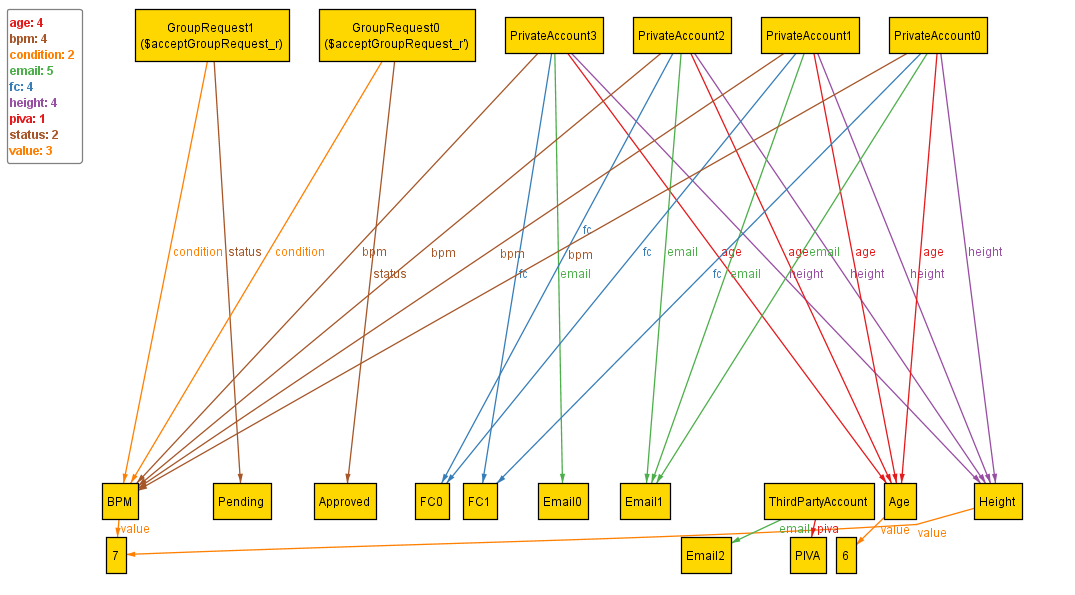
\includegraphics[width=\textwidth]{Alloy/groupRequest.png}
			\caption{Approved Group Request}
			\label{fig:groupg}
		\end{figure}

	\section{Efforts}
	In the following tables we will summarize the effort spent by each member of the team on the {\it RASD} Document.
		
		
	\begin{longtable}{| p{2 cm} | p{5 cm} | p{2 cm} |} 
			\hline
			{\bf Date} & {\bf Task} & {\bf Hours}\\
			\hline
			12/10/18 & Git setup & 2 \\
			19/10/18 & Pre-analysis & 2 \\
			24/10/18 & Complete Part 1 and organize following work & 2 \\
			25/10/18 & Product Functionalities and User Characteristics& 2 \\
			29/10/18 & Software, Hardware, Communication Interfaces & 1 \\
			30/10/18 & User Interfaces & 2 \\
			03/11/18 & Use Cases & 4 \\
			04/11/18 & Latex setup & 2 \\
			05/11/18 & Review Meeting & 3 \\
			06/11/18 & Use Case Diagrams, Scenarios & 1,5\\
			08/11/18 & Track4Run Use Cases & 2 \\
			09/11/18 & Goals, Requirements and Domain Assumptions Revision & 3 \\
			10/11/18 & Copy on Latex & 5 \\
			11/11/18 & Final Revision & 3 \\
			\hline
			& & {\bf Total} \\
			\hline
			& & 36,5 \\
			\hline
			\caption{Virginia Negri's effort}
		\end{longtable}
	
		\begin{longtable}{| p{2 cm} | p{5 cm} | p{2 cm} |} 
		\hline
		{\bf Date} & {\bf Task} & {\bf Hours}\\
		\hline
		12/10/18 & Git setup & 2 \\
		19/10/18 & Pre-analysis & 2 \\
		24/10/18 & Section 1.2 & 1 \\
		25/10/18 & Section 2.1 & 2 \\
		28/10/18 & Class Diagrams and State Charts & 2 \\
		30/10/18 & Section 3.4 & 1 \\
		01/11/18 & Section 3.3 & 1 \\
		04/11/18 & Section 2.1 refinement & 1 \\
		05/11/18 & Review Meeting & 3 \\
		05/11/18 & Class Diagrams updates and Scenarios & 1\\
		07/11/18 & Data4Help mockups & 4 \\
		09/11/18 & Track4Run Class Diagram & 1 \\
		10/11/18 & Track4Run mockups & 2 \\
		11/11/18 & Final Revision & 3 \\
		\hline
		& & {\bf Total} \\
		\hline
		& & 26 \\
		\hline
		\caption{Luca Molteni's effort}
	\end{longtable}
	
	\begin{longtable}{| p{2 cm} | p{5 cm} | p{2 cm} |} 
		\hline
		{\bf Date} & {\bf Task} & {\bf Hours}\\
		\hline
		12/10/18 & Git setup & 2 \\
		19/10/18 & Pre-analysis & 2 \\
		24/10/18 & Section 1.3 & 2 \\
		28/10/18 & Section 2.4 & 1,5 \\
		29/10/18 & Review & 0,5 \\
		30/10/18 & Section 3.5 & 2 \\
		03/11/18 & Section 4 & 4 \\
		05/11/18 & Review Meeting & 3 \\
		05/11/18 & Review & 1\\
		07/11/18 & Track4Run integration & 1 \\
		08/11/18 & Track4Run requirements & 3 \\
		09/11/18 & Track4Run review & 3 \\
		10/11/18 & Copy on Latex & 2 \\
		10/11/18 & Final Revision & 3 \\
		\hline
		& & {\bf Total} \\
		\hline
		& & 30 \\
		\hline
		\caption{Francesco Lorenzo's effort}
	\end{longtable}

	
\end{document}